%% ----------------------------------------------------------------
%% Thesis.tex -- MAIN FILE (the one that you compile with LaTeX)
%% ---------------------------------------------------------------- 

% Set up the document
\documentclass[a4paper,11pt,oneside]{Thesis}  % Use the "Thesis" style, based on the ECS Thesis style by Steve Gunn
\graphicspath{{Figures/}}  % Location of the graphics files (set up for graphics to be in PDF format)

% Include any extra LaTeX packages required
\usepackage[square, numbers, comma, sort&compress]{natbib}  % Use the "Natbib" style for the references in the Bibliography
\usepackage{verbatim}  % Needed for the "comment" environment to make LaTeX comments
\usepackage[final]{pdfpages} % Allows for importing of pdfs
\usepackage{listings} % Alows for code inclusions
\usepackage{float} % Float control for figures, tables, etc.
\usepackage[section]{placeins} % Fine-grain float placement control for float barriers

% Package and environment configuration
\lstset{language=c,breaklines=true,tabsize=3,aboveskip=1em,float=tbph} % Configure the Listings module for C code by default
\hypersetup{urlcolor=black, colorlinks=true}  % Colours hyperlinks in black to avoid distractions.
\setcounter{tocdepth}{2} % Only show Chapters, sections and sub-sections in the Table of Contents (no deeper nested sections)

% Custom command definitions
\newcommand{\superscript}[1]{\ensuremath{^{\textrm{#1}}}}
\newcommand{\subscript}[1]{\ensuremath{_{\textrm{#1}}}}

\begin{document}
%% ----------------------------------------------------------------
\frontmatter	  % Begin Roman style (i, ii, iii, iv...) page numbering

% Set up the Title Page
\title        {Embedded Bluetooth Stack}
\authors      {\texorpdfstring{\href{mailto:dean@fourwalledcubicle.com}{Dean Camera}} {Dean Camera}}
\addresses    {\groupname\\\deptname\\\univname}  % Do not change this here, instead these must be set in the "Thesis.cls" file, please look through it instead
\authordegree {Bachelor of Computer Science/ \\ Bachelor of Electronics Engineering}
\thesistype   {Undergraduate Thesis}
\date         {\today}
\subject      {}
\keywords     {}
\supervisor   {Prof. John Devlin}
\cosupervisor {Robert Ross}

\maketitle
%% ----------------------------------------------------------------
\setstretch{1.3}  % It is better to have smaller font and larger line spacing than the other way round

% Define the page headers using the FancyHdr package and set up for one-sided printing
\fancyhead{}  % Clears all page headers and footers
\rhead{\thepage}  % Sets the right side header to show the page number
\lhead{}  % Clears the left side page header
\pagestyle{fancy}  % Finally, use the "fancy" page style to implement the FancyHdr headers
%% ---------------------------------------------------------------- 
\addtotoc{Abstract}  % Add the "Abstract" page entry to the Contents
\abstract{
	\addtocontents{toc}{\vspace{1em}}  % Add a gap in the Contents, for aesthetics

	In modern electronic devices, both consumer and industrial, wireless technology is quickly becoming a
	must-have feature; wireless Bluetooth technology is now standard in almost all mobile phones, laptops and
	other devices. However, despite its prevalence, Bluetooth as a technology remains too expensive and/or
	impractical to integrate into embedded products and systems which lack large amounts of processing power
	and memory.
	
	While some existing embedded Bluetooth stacks are available, these remain expensive, limited, and/or
	closed-source, which otherwise prevent their use in applications where Bluetooth technology would be
	both desired and applicable.
	
	To combat this deficiency in the marketplace, the aim of this project is to designed and produce a free,
	open source, small footprint Bluetooth stack aimed to suit small embedded environments. This project will
	to allow for Bluetooth technology to be directly integrated into small scale products at a low cost, while
	remaining fully functional and extensible.
}

\clearpage  % Abstract ended, start a new page
%% ----------------------------------------------------------------
\setstretch{1.3}  % Reset the line-spacing to 1.3 for body text (if it has changed)

% The Acknowledgements page, for thanking everyone
\acknowledgements{
	\addtocontents{toc}{\vspace{1em}}  % Add a gap in the Contents, for aesthetics
	
	Special thanks to Robert Ross for his 3D modeling contributions to the project, without which the project's
	final robot design would be all the poorer. Also thanks to Ben Rampling for his expert assistance in reviewing
	the first revision of the project schematics.
	
	Thank you to the wider AVR community for their interest and support for the project, and to Matt from
	\textit{\href{http://www.micropendous.org}{Opendous Inc.}} for his generous contribution of the free
	\textit{``Micropendous''} AVR microcontroller boards used in the final robot prototype.
}

\clearpage  % End of the Acknowledgements
%% ----------------------------------------------------------------
\pagestyle{fancy}  %The page style headers have been "empty" all this time, now use the "fancy" headers as defined before to bring them back
%% ----------------------------------------------------------------
\pdfbookmark[0]{Contents}{Contents}
\lhead{\emph{Contents}}  % Set the left side page header to "Contents"
\tableofcontents  % Write out the Table of Contents
%% ----------------------------------------------------------------
\lhead{\emph{List of Figures}}  % Set the left side page header to "List of Figures"
\listoffigures  % Write out the List of Figures
%% ----------------------------------------------------------------
\lhead{\emph{List of Tables}}  % Set the left side page header to "List of Tables"
\listoftables  % Write out the List of Tables
%% ----------------------------------------------------------------
\phantomsection
\addcontentsline{toc}{chapter}{List of Code Listings}
\lhead{\emph{List of Code Listings}}  % Set the left side page header to "List of Code Listings"
\renewcommand\lstlistlistingname{List of Code Listings}
\lstlistoflistings
%% ----------------------------------------------------------------
\mainmatter
\pagestyle{fancy}

	\chapter{Overview}
\label{chp:overview}
\lhead{Chapter \ref{chp:overview}. \emph{Overview}}

In almost all modern portable consumer devices, Bluetooth plays a large role; it is available in the vast majority of mobile phones and their associated accessories, in cars, in laptops and, most recently, in mobile tablet PCs. Bluetooth as a technology gives system designers a low power wireless communications standard from the baseband up to the higher level abstract services, allowing implementing devices to communicate with one another in a manufacturer-independant manner. This freeing of consumers from the proprietary short range wireless solutions (such as \textit{ZigBee}) has helped make Bluetooth the wireless communication system of choice for many applications.

\section{Project Background}

Despite this ubiquity, Bluetooth remains firmly in the realm of systems containing large amounts of RAM and FLASH memories, processing power and---in many cases---full operating system stacks. For small-scale embedded devices with tiny 8-bit processors, clock speeds in the tens of MHz (or even less) and RAM measured in kilobytes, Bluetooth remains impractical; either due to its expense or the lack of suitable software.

However, existing solutions do exist. System designers can integrate off-the-shelf Bluetooth solutions in their products; small hardware modules containing the Bluetooth baseband and a fixed-function microprocessor. This microprocessor then handles the complex onion-like layers of the various Bluetooth stack components, off loading the computational load and implementation complexity from the main system processor. These modules are generally ridgid in their functionality however, making them unsuitable in applications where a specific or even custom Bluetooth service is required. In addition, such modules are generally significantly more expensive than the product's main processor, negating its cost/benefit ratio where a more powerful system processor could be substituted to manage the entire application including the Bluetooth component.

These turn-key modules are made all the less attractive when one considers the cost of a raw Bluetooth baseband IC module. Without an integrated processor to manage the software stack, these are generally available from multiple vendors at costs measured in the sub-US\$5 range. This indicates that the main cost of the complete modular solutions lies not in the physical hardware, but the IP of the Bluetooth software stack. If such a stack could be made widely available for use in embedded systems, this fixed-cost vendor lock-in could be avoided and cheaper Bluetooth enabled systems developed for both hobbyist and commercial use.

\section{Project Brief}

To help fill the identified gap in the marketplace for a cheap, open source Bluetooth stack aimed at the low to mid-range embedded market, it is proposed that a new stack be designed from scratch specifically for this market segment. This stack would offer a base amount of functionality suitable for integration into new or existing embedded systems, to extend the system functionality to include wireless Bluetooth communications.

At a minimum, a functional Bluetooth stack needs to have at least four components:

\begin{enumerate}
	\item A \textbf{Physical Data Transport layer} to and from a connected Bluetooth physical baseband transceiver IC
	\item An implementation of the Bluetooth specification's \textbf{HCI layer} for the establishment and management of physical connections to and from remote devices
	\item An implementation of the Bluetooth specification's \textbf{L2CAP layer} for the establishment and management of logical channels within an established connection
	\item One of more \textbf{Bluetooth Services} on top of the L2CAP layer to implement functionality such as the Service Discovery Protocol (SDP)
\end{enumerate}

These components, when put together, form the basis of a minimal Bluetooth stack \emph{(see Figure \ref{fig:btstack})}. Additional services may or may not be added on top of the stack in parallel with the mandatory SDP protocol to expose local device functionality and interact with remote devices.

\begin{figure}[H]
	\centering
		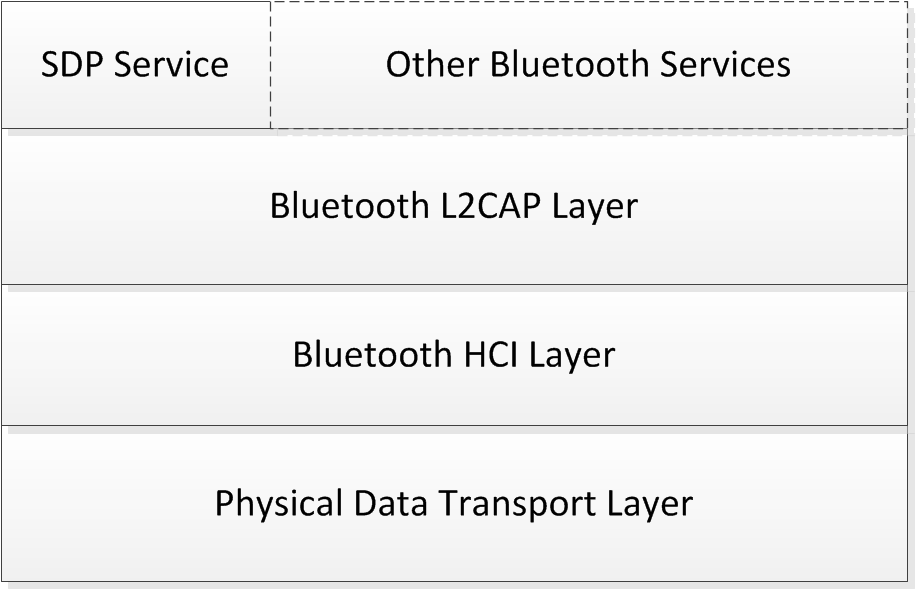
\includegraphics[width=80mm]{BluetoothStack.png}
	\rule{35em}{0.5pt}
	\caption[Diagram of a typical Bluetooth Stack]{Diagram of the basic components which form a typical Bluetooth Stack}
	\label{fig:btstack}
\end{figure}

As the usefulness of an abstract piece of software is inherently low without a suitable demonstration platform, a second component of the project will be to design, develop and prototype a functional and practical device which uses the created stack. It is proposed that this hardware component be in the form of a small \textit{``ExplorerBot''} robot (see Figure \ref{fig:robotoutline}), able to stream local sensor data wirelessly to a remote PC for real-time graphing purposes, and to allow for remote wireless control over a Bluetooth link to a consumer Bluetooth control device, such as a current generation Game Console controller (\textit{Wii} or \textit{Playstation 3}). If possible, these two functions should be combined to allow for multiple simultaneous connections, allowing for remote control at the same time as the sensor data is logged remotely.

\begin{figure}[H]
	\centering
		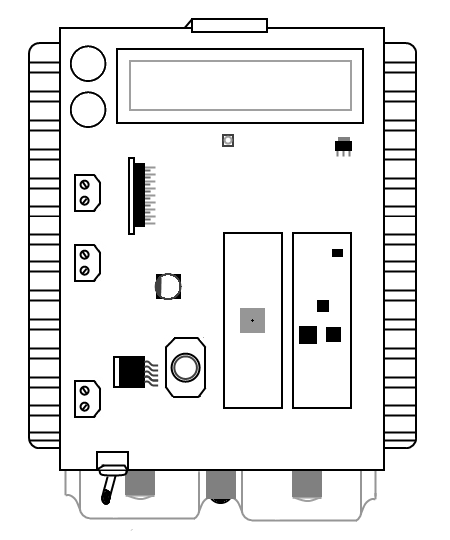
\includegraphics[width=60mm]{RobotOutline.png}
	\rule{35em}{0.5pt}
	\caption[Diagram of the proposed robot]{Diagram of the proposed robot platform.}
	\label{fig:robotoutline}
\end{figure}

With the combination of the software \emph{(the stack)} and hardware \emph{(the robot)} components of this project, the final design should offer a complete system and test platform which can be reproduced wholesale, modified to suit a particular application or used as a reference implementation for other projects.

\section{Design Goals}

The design goals of the project were split into two distinct parts, consisting of the software Bluetooth Stack implementation, and the physical robot hardware design. This separation of the testing platform hardware goals from those of the logical Bluetooth stack allowed for the clearest representation of the project as a whole.

\subsection{Software Goals}

For such a stack to be useful in an embedded environment, it must be able to conform to the restrictions such an environment imposes. Specifically, the completed stack must minimize its compiled and working set footprints, reduce or eliminate the need for dynamic memory allocation, and minimize its hardware dependencies to suit as wide a range of processors of differing capabilities as possible.

The design goals of the complete software stack were therefore set to:

\begin{itemize}
	\item Use as little RAM as possible
	\item Compile to as small a binary as is practical
	\item Offer a framework upon which services can be added to suit a particular application
	\item Provide asynchronous events to which the user application can respond to
	\item Allow for a variable number of simultaneous connections and logical channels to/from remote devices
	\item Have no requirement for dynamic memory allocation on the heap
	\item Allow for integration into an optional RTOS, but support stand-alone operation
	\item Be fully decoupled from the physical transport to the Bluetooth Adapter
	\item Be endian-correct regardless of native processor endianness
	\item Maintain a level of compatibility with Bluetooth Version 2.1 specification as maintained by the Bluetooth \textit{Special Interest Group} (SIG)
\end{itemize}

While at the point of the project's design and development a newer Bluetooth 3.0 version standard was available, a decision was made to implement the slightly older---and far more popular---version 2.1 of the Bluetooth specification. This decision was made due to the abundance of cheap Bluetooth 2.1 compatible hardware already of the market (and, conversely, the lack of cheap and widely available Bluetooth 3.0 hardware). In addition, the aim of the project was set to produce a \textit{compatible} rather than fully \textit{compliant} stack, due to the significantly increased development complexity of the latter for little additional benefit.

\subsection{Hardware Goals}

To make a useful, visual and functional testing platform, a decision was made to produce a small, battery powered robot. This robot would serve as both a testing platform for the completed stack to verify its correct operation in a real-world environment during development, and to function as a reference application of the completed stack.

In order to fully demonstrate the capabilities of the Bluetooth stack, the robot would have to include both locally initiated Bluetooth connections, as well as accept remotely initiated connections. In addition to this requirement, data would have to be both received and sent to and from a remote device to demonstrate full duplex communications.

A set of design goals was thus created for the robot:

\begin{itemize}
	\item Allow the user to initiate a connection to a remote device via the robot
	\item Accept incoming connections from remote Bluetooth devices, including some level of authentication
	\item Consume data received from remote Bluetooth device(s) via one or more Bluetooth services
	\item Produce data to be transmitted to remote Bluetooth device(s) via one or more Bluetooth services
	\item Visually indicate status and debug messages via a display mechanism, for debugging
	\item Allow for the robot to be remotely driven via a set of PWM controlled DC motors
\end{itemize}

% TODO

	\chapter{Existing Implementations}
\label{chp:existingimp}
\lhead{Chapter \ref{chp:existingimp}. \emph{Existing Implementations}}

Before work was started on the proposed software Bluetooth stack implementation, the existing field of Bluetooth stacks (both commercial and non-commercial) were evaluated to determine what capabilities are being offered.

\section{Classes of Existing Stacks}

During the course of the project background research into existing Bluetooth stacks, two distinct classes of stack were observed, each with distinct assumptions and capabilities:

\begin{itemize}
	\item \textbf{Operating System based Stacks}, which assumed that they would be run on top of a complex full-featured OS, containing a kernel- and user-space, virtualized memory, synchronisation primitives, etc.
	\item \textbf{Embedded Stacks}, which assumed no OS was present, but nevertheless made assumptions as to the environment's capabilities for dynamic memory allocation
\end{itemize}

These two classes of stacks show two possible approaches to an implementation; one, the designer may write a stack around an existing Operating System API, or two, the designer can assume a "freestanding" or "bare metal" environment, with either no, or only a minimal, RTOS being present.

\section{Existing Bluetooth Stacks}

Below the discovered existing Bluetooth stacks are listed in parametric form for each class of stack for ease of reference.

\subsection{Operating System Stacks}

\begin{table}[H]
	\begin{center}
		\begin{tabular}{ | l | l | l |}
			\hline
			\textbf{Stack Name}	& \textbf{Operating System}	& \textbf{Commercial} \\ \hline

			FreeBSD Stack		& FreeBSD	& No	\\ \hline
			Affix Stack			& Linux		& No	\\ \hline
			BlueZ Stack			& Linux		& No	\\ \hline
			Apple Stack			& MacOS		& Yes	\\ \hline
			BlueFritz! Stack	& Windows	& Yes	\\ \hline
			CSR Harmony Stack	& Windows	& Yes	\\ \hline
			FreeBT Stack 		& Windows	& No	\\ \hline
			Microsoft Stack		& Windows	& Yes	\\ \hline
			Toshiba Stack		& Windows	& Yes	\\ \hline
			Widcomm Stack		& Windows	& Yes	\\ \hline
		\end{tabular}
		\caption[Existing Operating System Bluetooth Stacks]{Parametric table of existing OS based Bluetooth stacks}
		\label{tab:osbtstacks}
	\end{center}
\end{table}

As expected, the vast majority of existing OS based Bluetooth stacks are targeted towards the Microsoft Windows operating system, due to its large market share. In almost all cases, the existing stacks were found to support a rich number of Bluetooth services, in both device and server roles. While the majority of the Bluetooth stacks on the market are commercialized (i.e. require payment or hardware purchase for a license to use them) there are still several free and open source stacks available for the various Linux and BSD kernels.

% TODO

\subsection{Embedded Stacks}

\begin{table}[H]
	\begin{center}
		\begin{tabular}{ | l | l |}
			\hline
			\textbf{Stack Name}	& \textbf{Commercial} \\ \hline

			BlueCode+ Stack		& Yes	\\ \hline
			BlueLet Stack		& Yes	\\ \hline
			BlueMagic Stack		& Yes	\\ \hline
			Bluetopia Stack		& Yes	\\ \hline
			BTStack Stack		& No	\\ \hline
			ClarinoxBlue Stack	& Yes	\\ \hline
			CSR Synergy Stack	& Yes	\\ \hline
			EtherMind Stack		& Yes	\\ \hline
			Jungo BTware Stack	& Yes	\\ \hline
			lwBT Stack			& No	\\ \hline
			Mecel Betula Stack	& Yes	\\ \hline
			Symbian OS Stack	& Yes	\\ \hline
		\end{tabular}
		\caption[Existing Embedded Bluetooth Stacks]{Parametric table of existing embedded Bluetooth stacks}
		\label{tab:embbtstacks}
	\end{center}
\end{table}

Contrasting with the OS based stacks discussed previously, almost all Bluetooth stacks aimed at the embedded market today were found to be exclusively commercialized, requiring large payments and license agreements before they could be integrated into existing designs. Of note in this area are the \textit{BTStack} and \textit{lwBT} embedded Bluetooth stacks, which were both found to be both free and open source, but suffered from the constraints of RTOS dependencies in the case of the former, and incompleteness in the case of the latter.

% TODO

	\chapter{Bluetooth Stack Implementation}
\label{chp:btstackimp}
\lhead{Chapter \ref{chp:btstackimp}. \emph{Bluetooth Stack Implementation}}

The development of the Bluetooth stack followed a bottom-up development methodology, designing and writing each software layer in sequence from the lowest layer first, to the highest and most abstracted layers last. This sequence ensured that each layer was functionally correct and could be verified before the higher layers were implemented. This suited the development of the Bluetooth stack---and, indeed, most software stacks---as each higher software layer is dependant solely on lower logical layers in the stack.

\section{Software Overview}

The software layers implemented in the completed Bluetooth stack are shown in Figure \ref{fig:completedbtstacklayers}.

\begin{figure}[tbph]
	\vspace{1em}
	\centering
		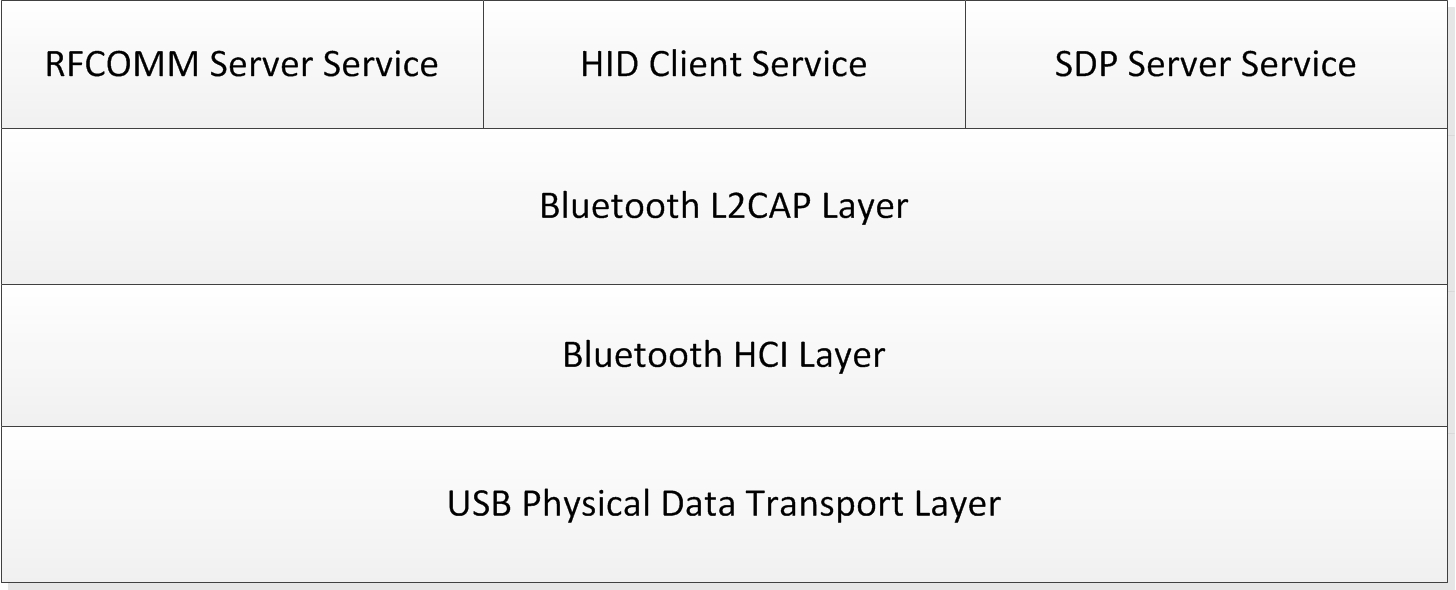
\includegraphics[width=100mm]{CompletedBluetoothStack.png}
	\rule{35em}{0.5pt}
	\caption[Diagram of the completed Bluetooth stack layers]{Diagram showing the completed layers of the Bluetooth stack.}
	\label{fig:completedbtstacklayers}
\end{figure}

Each software layer was implemented as a seperate pair of source code module files, written in the C language and targeted towards the C99 language specification. Configuration for the stack is located in the file \texttt{BluetoothCommon.h}, which must be included in the user application to operate the stack.

% TODO

\section{Design Restrictions}

A number of design restrictions were placed on the development of the Bluetooth stack; these ensured that the completed stack remained modular, extensible and suitable for integration in a wide range of embedded systems with various capabilities, and conversely, limitations. As an unfortunate but expected side effect, a number of these restrictions complicated the software development process significantly.

\FloatBarrier
\subsection{No Heap Memory Allocations}

The largest restriction placed on the stack design was the requirement of static and stack allocated memory allocation only --- no dynamic heap allocated memory was to be used via the usual \lstinline{malloc()} and \lstinline{free()} functions from the \texttt{libc} library. Most embedded environments contain three types of memory allocations:

\begin{enumerate}
	\item \textbf{Static Allocations}, including global variables and \lstinline{static} qualified variables.
	\item \textbf{Stack Allocations}, automatically populated to store local automatic variables, function paramaters, return addresses, etc.
	\item \textbf{Heap Allocations}, persistant dynamic allocations manually managed by the user application.
\end{enumerate}

However, for significantly memory constrained systems, heap allocations are generally avoided due to the possibility of memory fragmentation; large numbers of differently-sized allocations and deallocations may cause fragmented holes to appear within the heap environment, causing allocation exhaustion to occur even if sufficient (raw) memory is available for an allocation request. In addition, dynamic memory complicates the formal analysis of a program, making memory requirements harder to judge, and thus harder to determine whether a given set of firmware will operate correctly within a specified environment without further in-depth analysis. In large embedded environments (ones with virtual memory management, and/or a large heap space) these problems are less of an issue and dynamic memory may be preferable for its simplicity.

The design of embedded stacks based on a no-heap-allocation strategy is a complex one, requiring certain trade-offs to be made. In the case of the Bluetooth stack presented here, a major side-effect of this decision was the need to fix the maximum number of simultaneous HCI device connections, L2CAP channel connections, and other queue- and list-like data structures within each instance of the stack. A major downside to this approach is the increased complexity of packet buffering and re-assembly, as fixed-size buffers must be used.

\FloatBarrier
\subsection{Endianness Correction}

A second complication based on the physical constraints from the execution environment is the native endianness of the processor hardware, i.e., the order in which multiple-byte data values are stored inside the processor. Depending on the execution architecture, data values may be represented in Big Endian (most significant byte at the lowest address) or Little Endian (least significant byte at the lowest address) format within the CPU. Data transmitted and received at the local device to remote device boundary must undergo a encoding conversion if the endianness of the source and sink do not match.

In the case of the Bluetooth specification, this was further complicated by the various layers; some layers used Little Endian encoding for exchanged data, while others selected Big Endian. To perform the correct encoding/decoding on each platform, a set of conversion macros were implemented at points where multi-byte values were exchanged. This ensured that regardless of the native endian format of the architecture the stack is compiled to, multi-byte values will be interpreted correctly.

\FloatBarrier
\subsection{Physical Transport Independance}

As the Bluetooth 2.1 specification outlines a several possible physical transports of HCI packets between the Bluetooth transceiver silicon and the application microcontroller, it was important that the physical transport layer be made independant from the rest of the stack. By making no assumptions about the form of transport protocol used to transfer packets to and from the attached Bluetooth silicon, the user application is free to implement their own transport mechanism without having to modify the internals of the stack. One instance of the stack may run across a USB connection to an attached Bluetooth module, while another may simultaneously connect to the microcontroller over a USART link.

\FloatBarrier
\subsection{Bluetooth Specification Compatibility}

For a software stack to be suitable for general use, it must be designed around, and undergo a series of tests to ensure compatibility with, a particular version of the protocol specification. Without a fixed version of a specification, correctness of the finished stack and compatibility with other implementations of the same technology cannot be assured.

As a \textit{compliant} stack would require extensive development and expensive certification procedures, the stack was instead aimed to be \textit{compatible} with version 2.1 of the Bluetooth specification. This subtle difference in the terminology indicates a large difference in the restrictions around the exact implementation. While a \textit{compliant} stack must be verified against the entire specification and rigorously tested to ensure exact conformance, a \textit{compatible} must only work with (most) other devices implementing their own compliant or compatible stacks of the same protocol version.

In the future the stack could be made conformant if desired, however for the purposes of the project only protocol compatibility was tested.

\FloatBarrier
\subsection{Multiple Stack Instances}

For maximum utility, the stack was designed to allow for multiple simultaneous stack instances. This was implemented to allow for unusual Bluetooth usage scenarios where more than one tranceiver is desirable in the one system, either for security, wireless signal coverage or bandwidth reasons. Each physical transceiver is allocated a logical stack instance, capable of sustaining one or more simultaneous connections, and one or more logical channels between devices. This flexibility ensures that the majority of usage scenarios are covered by the stack's implementation.

Code-wise, the multiple stack functionality is implemented as a common first parameter to all functions within the stack, \lstinline{BT_StackConfig_t* const StackState}. This parameter is used to pass around a reference to the stack instance being operated upon, and is somewhat analagous to the \lstinline{this} property in C++ classes, if the entire stack was wrapped in a single class. As the stack was written in the C language which lacks Object Orientated language capabilities, this form of basic polymorphism was implemented manually. For each physical tranceiver, the user application is expected to declare a new instance of the \lstinline{BT_StackConfig_t} structure within their code, and pass this to the main Bluetooth stack management routines (see Listing \ref{lst:stackconfig}).

\lstinputlisting[float=tbph,caption={Configuration example of a Bluetooth stack instance.},label={lst:stackconfig}]{./Figures/StackConfig.c}

\FloatBarrier
\subsection{Multiple Simultaneous Connections and Channels}

The HCI connections and L2CAP channels for each stack instance are implemented as an pair of object pools within the \lstinline{BT_StackConfig_t} structure; L2CAP channel objects within the pool are shared amongst all established HCI connections --- for example, one HCI connection may use all the available L2CAP channels, or two connections may share the pool equally. This design decision allows the full pool of L2CAP channel objects to be used by the stack regardless of the HCI connection requesting them. Figure \ref{fig:stackobjectpools} illustrates a single stack instance with a typical usage scenario, with two of the stack's HCI objects containing established connections, each with several L2CAP channel objects associated with the connection from the channel object pool.

\begin{figure}[tbph]
	\vspace{1em}
	\centering
		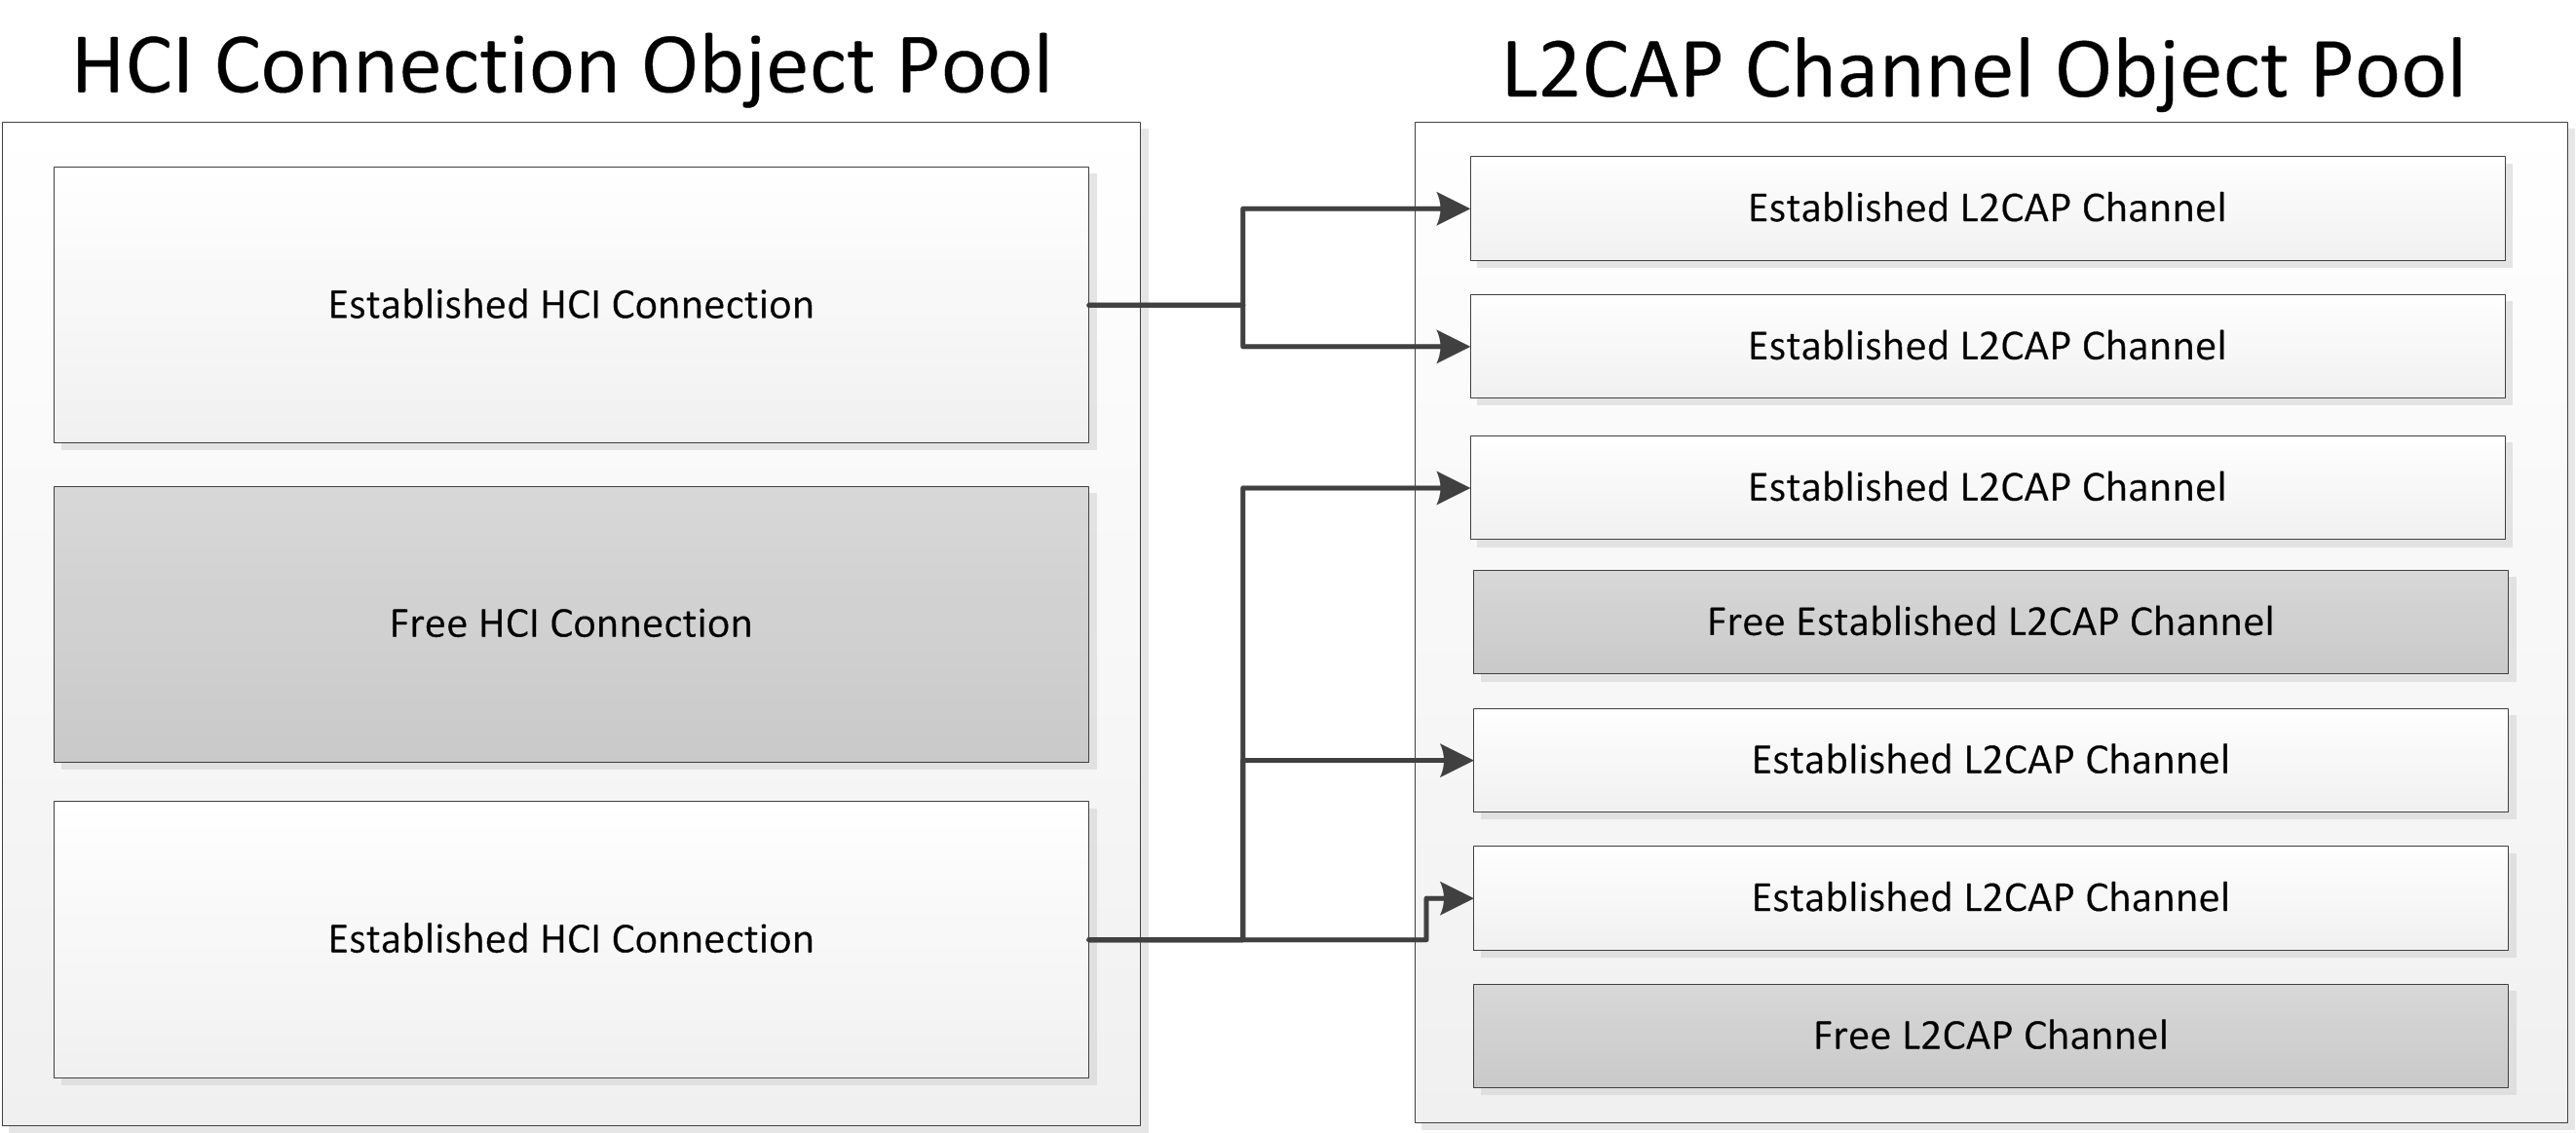
\includegraphics[width=140mm]{StackObjectPools.png}
	\rule{35em}{0.5pt}
	\caption[Diagram of the Bluetooth stack instance object pools]{Diagram showing the HCI Connection and L2CAP object pools within a stack instance.}
	\label{fig:stackobjectpools}
\end{figure}

To positively link one used L2CAP channel instance to its parent HCI connection object, the HCI connection's \texttt{handle} property is stored in the L2CAP channel object as a primary key. This handle value, allocated uniquely by the external Bluetooth HCI controller silicon when a new HCI connection is made, is then used to locate the HCI connection object within a stack instance from an established channel instance. While a pointer to the parent HCI object would offer a faster method of locating the associated HCI connection, this would tightly couple the HCI layer with the L2CAP layer as the former would need to alter the latter's objects if and when HCI connections are terminated.

As the stack does not use heap-based dynamic memory allocation, this approach ensures that the stack contains similar levels of flexability to a dynamically allocated object approach, with only a minimal overhead. The maximum size of each object pool is set via the Bluetooth Stack's \lstinline{BT_MAX_DEVICE_CONNECTIONS} and \lstinline{BT_MAX_LOGICAL_CHANNELS} configuration defines.

\FloatBarrier
\subsection{Minimal Memory Usage}

While large embedded systems may run the completed Bluetooth stack, the design decisions made during its development were primarily aimed at ensuring the best performance and smallest footprint in very low powered microcontrollers. This resulted in the stack being optimised for small systems; only the minimal attributes required to establish and maintain connections are stored by the stack. One example of these optimizations is in the event system (described in detail later in this chapter) implementation: rather than implementing a callback registration system for each event, named callbacks are used instead. Various portions of the Bluetooth stack expect the user application to provide callback and event functions using names and prototypes defined in the stack header files.

This named callback function system reduces the memory footprint of the stack, as the callback addresses do not need to be stored in RAM at runtime, and the compiler does not need to inflate the binary with additional functions to manage the callback function registrations.

\section{Software Layer Implementation}

% TODO

\FloatBarrier
\subsection{Physical Transport}

% TODO

\FloatBarrier
\subsection{HCI Layer}

% TODO

\FloatBarrier
\subsection{L2CAP Layer}

% TODO

\FloatBarrier
\subsection{Bluetooth Services}

% TODO

\FloatBarrier
\subsubsection{SDP Service}

% TODO

\FloatBarrier
\subsubsection{HID Service}

% TODO

\FloatBarrier
\subsubsection{RFCOMM Service}

% TODO

\section{Integration into User Applications}

% TODO

\FloatBarrier
\subsection{Events and Callbacks}

\begin{figure}[tbph]
	\vspace{1em}
	\centering
		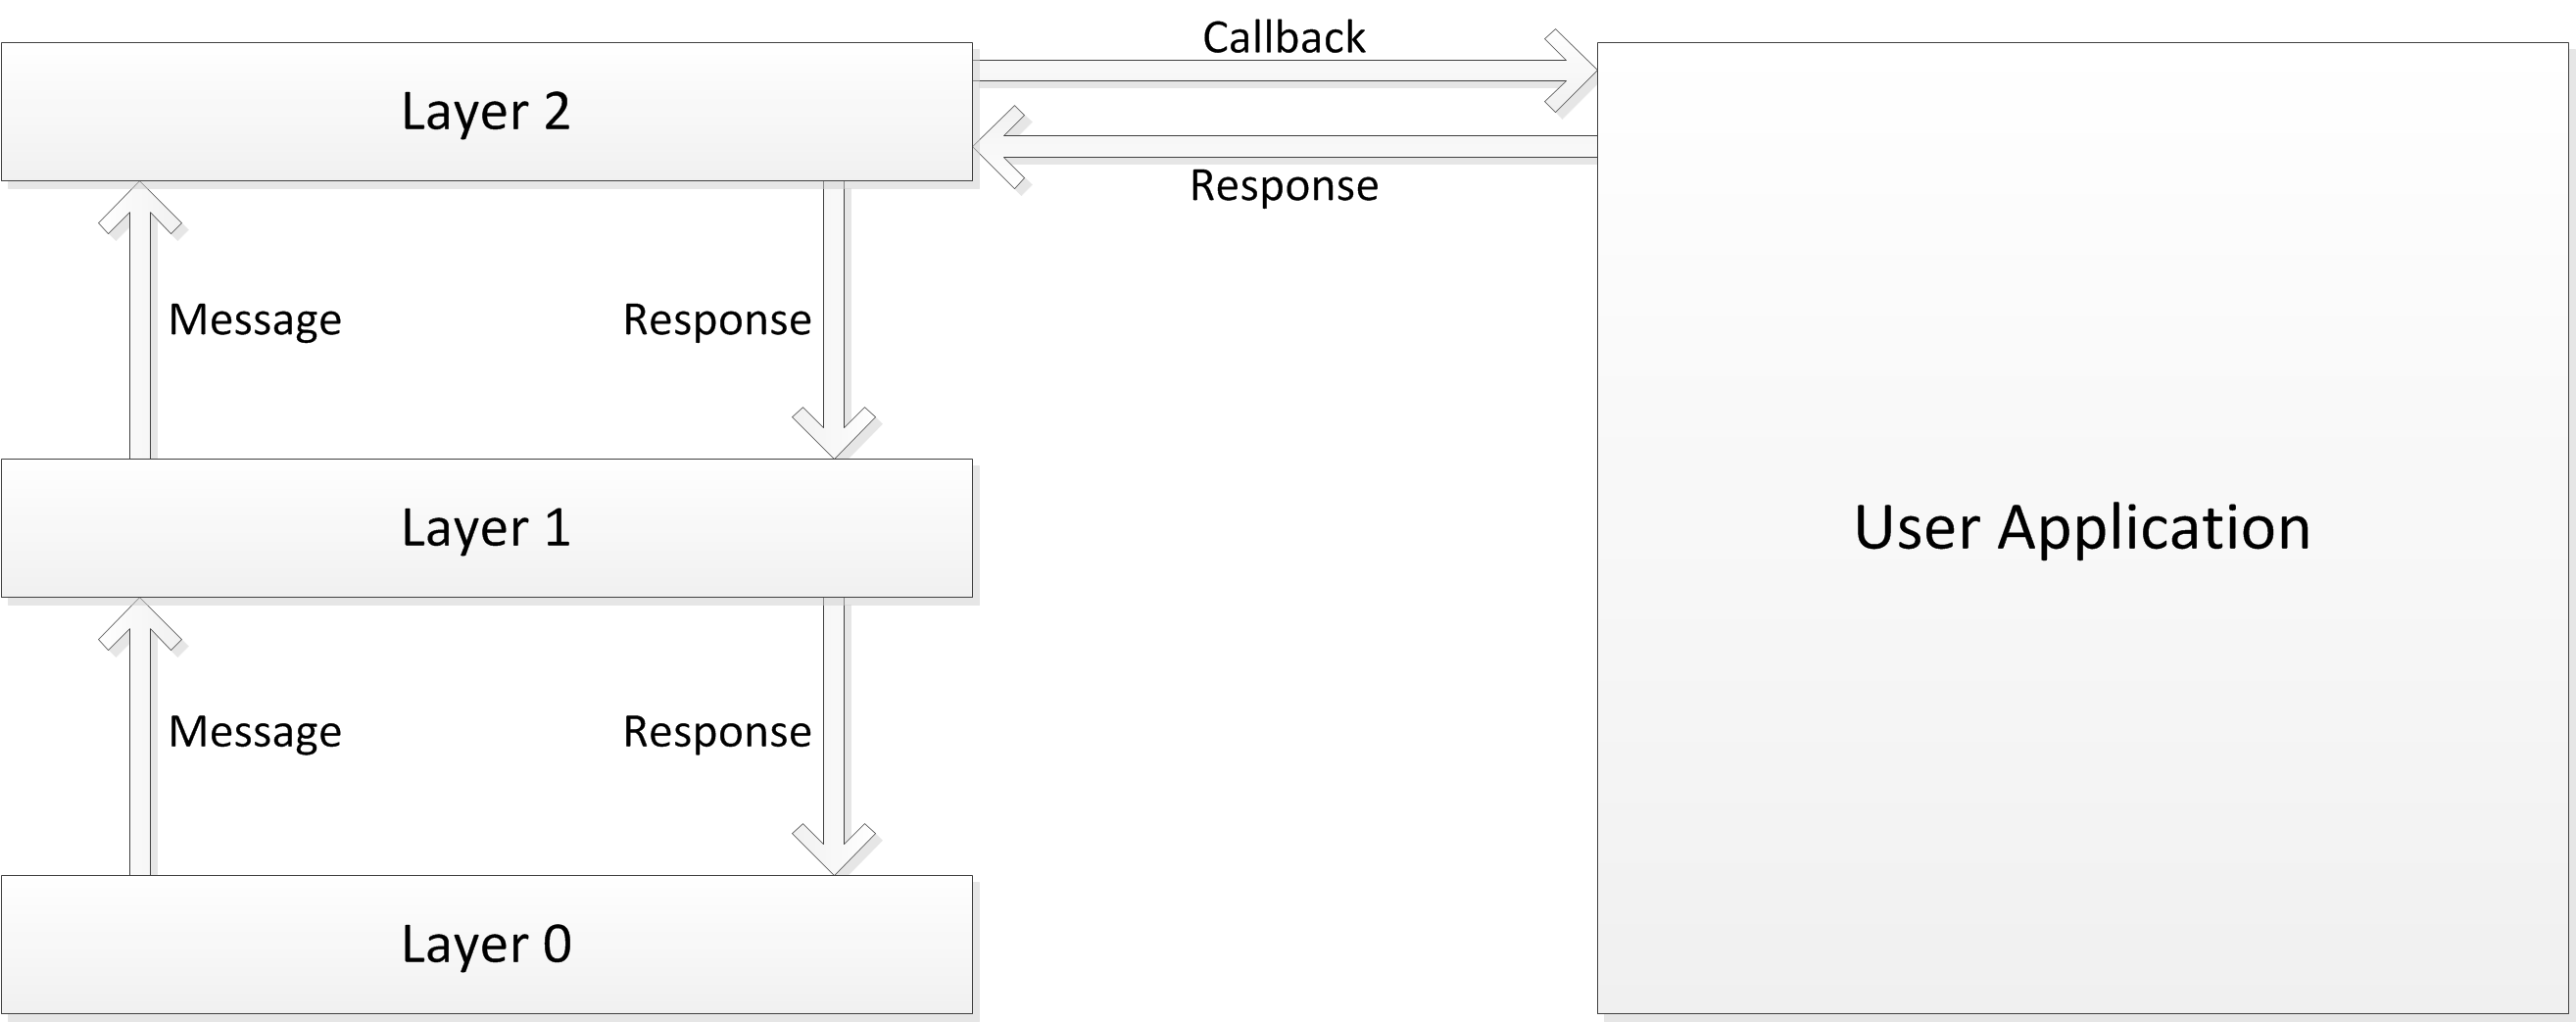
\includegraphics[width=140mm]{MessageResponseCallback.png}
	\rule{35em}{0.5pt}
	\caption[Diagram of the Message, Response and Callback sequence]{Diagram showing the Message, Response and Callback sequence of a typical software stack when passing a message and response through several intermediate layers.}
	\label{fig:messageresponsecallback}
\end{figure}

% TODO

\FloatBarrier
\subsection{Management Functions}

% TODO
	\chapter{Robot Hardware Implementation}
\label{chp:robothwimp}
\lhead{Chapter \ref{chp:robothwimp}. \emph{Robot Hardware Implementation}}

To help demonstrate the usefulness of the stack in a practical manner, a robot was designed and constructed. This robot, named the \emph{ExplorerBot}, was then used to give a practical reference implementation of a full project utilizing the custom embedded Bluetooth stack in a real-world environment.

\section{Hardware Overview}

The completed robot design for the project contains many useful capabilities for both mobility and exploration. Built on top of a pre-fabricated (including raw DC motors and gearing) ``Tank'' style hobby robot base, the \emph{ExplorerBot} robot implements the following features:

\begin{itemize}
	\item Primary switch-mode based 5V power supply
	\item Secondary LDO based 3.3V power supply for attached sensors
	\item 2x16 Alphanumeric LCD Screen for feedback to the user
	\item Two momentary pushbuttons for user control
	\item One RGB status LED for basic status feedback
	\item Dual PWM motor control system, with variable speed and direction of DC motors
	\item Level converted I\textsuperscript{2}C bus for the attached sensor(s)
	\item Support for the Atmel \textit{Inertial One} and \textit{Pressure One} sensor boards
	\item High intensity LED based headlights for frontal illumination
	\item Piezo speaker for audio feedback and ``horn'' like functionality
	\item Atmel \textit{AT90USB1287} 8-Bit Microcontroller
	\item External 128KB SRAM for temporary storage of packets to and from the Bluetooth adapter
\end{itemize}

The complete robot design was created in the \textit{Altium Designer} software, including both the schematic design and board routing. Surface mount components were chosen where possible to reduce the board space required, and two board layers used as this proved to offer the lowest cost/time ratio. The final board design measured 10cm x 15cm, however much of this board space is relatively unused; with optimization, this board space could be reduced considerably.

To get the best results in the construction of the robot, the boards were manufactured commercially. This process ensured the manufactured board's quality while also provided solder mask and silk-screen to reduce the potential for error in the robot's construction.

\section{Hardware Modules}

In the section, the various hardware components of the constructed robot are detailed at the block level. Figure \ref{fig:robotblockhw} below illustrates how the various hardware blocks that comprise the robot connect together to make the final design.

\begin{figure}[H]
	\vspace{1em}
	\centering
		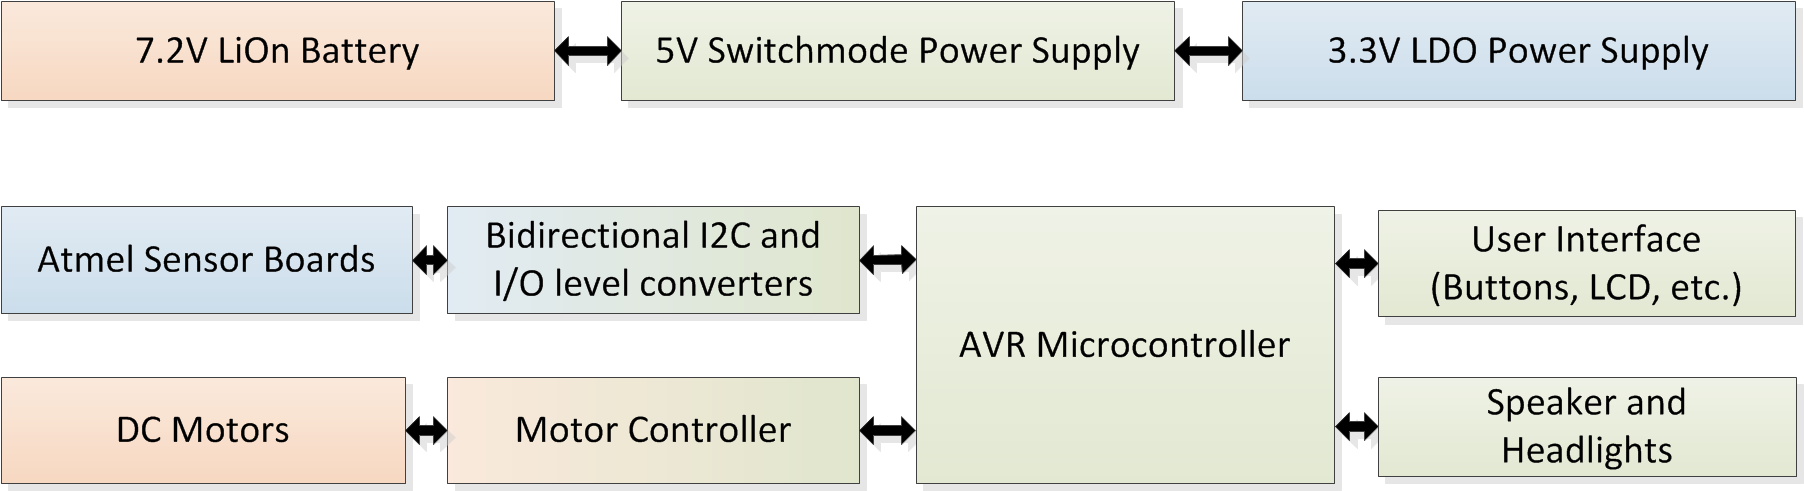
\includegraphics[width=140mm]{HardwareBlockDiagram.png}
	\rule{35em}{0.5pt}
	\caption[Hardware Block Diagram]{Robot Hardware Block Diagram}
	\label{fig:robotblockhw}
\end{figure}

\FloatBarrier
\subsection{Microprocessor}

Due to the author's familiarity with the Atmel line of \textit{AVR} branded microcontrollers, one of the available models in this line-up was chosen to serve in the robot as the main processor, the AT90USB1287. This 8-bit microcontroller contains 128KB of non-volatile FLASH memory for program storage, 4KB of non-volatile EEPROM for user application parameter storage and 8KB of internal SRAM for scratch memory. A 16MHz clock (provided by an external crystal) was selected for the design as this offered the fastest possible speed the chip was capable of, while still allowing the hardware USB host controller inside the chip to function normally. As a trade-off, this higher clock speed put a constraint on the main logic level voltage; at 16MHz, the AVR microcontroller required 5V to be within the datasheet's specifications.

As the AT90USB1287 and associated USB components are difficult to source in single quantities at reasonable prices, the use of a commercial breakout module containing this chip was selected instead: the \textit{Micropendous-A} board (see Figure \ref{fig:micropendous}). This board contains the surface mount AVR microcontroller and associated USB components, along with an external 128KB SRAM chip attached to the AVR's external memory bus interface. As the Bluetooth stack required a large temporary buffer for incoming fragments, the selection of this board proved ideal for the intended purpose.

\begin{figure}[tbph]
	\vspace{1em}
	\centering
		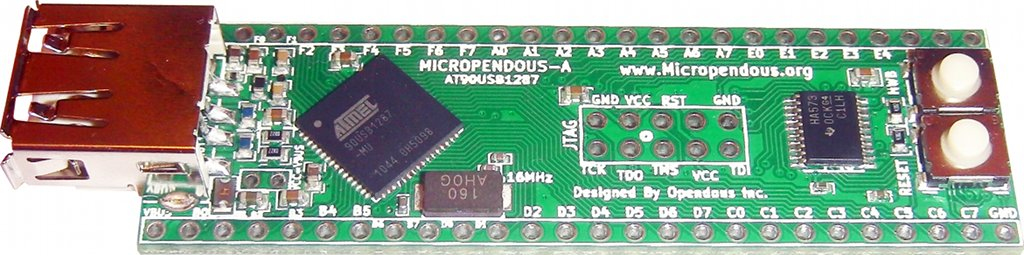
\includegraphics[width=100mm]{MicropendousA.jpg}
	\rule{35em}{0.5pt}
	\caption[Micropendous-A Board]{The Micropendous-A Board (Image courtesy \textit{Opendous Inc.})}
	\label{fig:micropendous}
\end{figure}

\FloatBarrier
\subsection{Primary Power Supply}

As the vast majority of the robot's hardware operated at a fixed 5V level, a power supply was required to reduce the Lithium Ion battery's raw 7.2V (nominal) voltage down to the 5V level needed to power the various components. Due to the use of battery power in the project, reducing power consumption where possible was a large concern; thus, a switch-mode design was chosen for maximum voltage conversion efficiency. A conventional linear regulator was considered for the design, but rejected due to the prohibitively large amount of power this would waste (approximately .45W, assuming an average 200mA operating current).

The regulator selected for the project was the M2595S-5.0, a fixed-function switch-mode regulator capable of outputting a fixed 5V rail at loads of up to 3A. While the robot design would not consume even a fifth of this power, the overhead in the specifications ensured that the power supply would remain robust and the output within the tolerances of the system components regardless of the load demanded. The exact schematic used in the final robot power supply design (see Figure \ref{fig:mainpowersupply}) was taken from the regulator component's datasheet to ensure correct operation.

\begin{figure}[tbph]
	\centering
		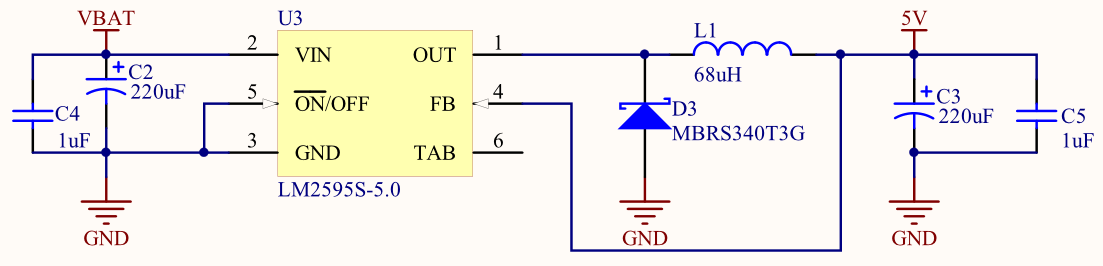
\includegraphics[width=150mm]{MainPowerSupply.png}
	\rule{35em}{0.5pt}
	\caption[Main Power Supply Schematic]{Schematic of the robot's main 5V switch-mode power supply.}
	\label{fig:mainpowersupply}
\end{figure}

\FloatBarrier
\subsection{User Interface}

For interaction with the user, the robot contains several components, detailed below.

\FloatBarrier
\subsubsection{RGB Status LED}

For primary status indication, a surface mount RGB LED indicates the current status of the robot. Due to a lack of free PWM channels on the AVR microcontroller, the three LED sub-components are wired directly to standard GPIO ports. While this design prevented PWM fading of the individual LED subcomponents to produce a many-bit custom colour from the LED, a three bit colour space is possible giving a total of 8 possible colour states (see Table \ref{tab:rgbcolours}). For the purposes of the created robot, this is in practice more than enough for basic status indication.

\begin{table}[H]
	\begin{center}
		\begin{tabular}{ | l | l | l | l |}
			\hline
			\textbf{R}	& \textbf{G} & \textbf{B} & \textbf{Output Colour} \\ \hline

			0 & 0 & 0 & Off		\\ \hline
			0 & 0 & 1 & Blue	\\ \hline
			0 & 1 & 1 & Cyan	\\ \hline
			0 & 1 & 0 & Green	\\ \hline
			1 & 1 & 0 & Magenta	\\ \hline
			1 & 0 & 0 & Red		\\ \hline
			1 & 0 & 1 & Yellow	\\ \hline
			1 & 1 & 1 & White	\\ \hline
		\end{tabular}
		\caption[RGB LED Colour Table]{Table of the possible output colours of the RGB LED, with binary inputs.}
		\label{tab:rgbcolours}
	\end{center}
\end{table}

To achieve a somewhat uniform brightness, the three LEDs were adjusted with current limiting resistors to consume an equal amount of current (approx. 5mA) despite differing forward voltages. As the RGB status LED shares the same I/O pins as the microcontroller's JTAG port for programming and debugging, the RGB LED's common anode was connected via a removable wire link (see Figure \ref{fig:rgbwirelink}) to ensure that it could be taken out-of-circuit if it proved to interfere with the external hardware debugger during development.

\begin{figure}[tbph]
	\centering
		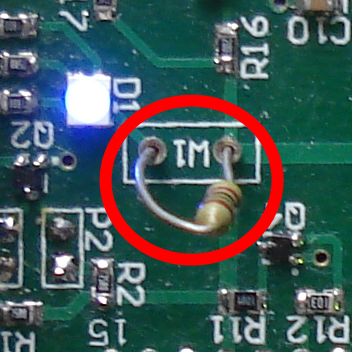
\includegraphics[width=40mm]{RGBWireLink.png}
	\rule{35em}{0.5pt}
	\caption[Close-up of the RGB LED's Removable Wire Link]{Close-up of the removable wire link used to disable the RGB status LED to prevent conflicts with the JTAG lines during programming/debugging.}
	\label{fig:rgbwirelink}
\end{figure}

\FloatBarrier
\subsubsection{LCD Display}

For situations where more information needs to be communicated to the user than is possible via the RGB status LED, a 16x2 Alphanumeric LCD display---compatible with the well known Hitachi HD44780 chipset---was added to the design. Due to the limited number of GPIO pins available on the microcontroller, the LCD was wired in 4-bit mode, with the lower 4 data pins on the LCD being wired directly to ground (see Figure \ref{fig:lcdschematic}). While this doubled the time required to send a byte to the LCD (as bytes then need to be split into a pair of 4-bit nibbles) the high speed of the processor meant that in practice this had little or no effect to the overall speed of the system.

The LCD backlight was wired through a driver transistor to a spare PWM channel on the AVR microcontroller, allowing for 8-bit PWM brightness control to reduce power consumption of the backlight when not in use. As the LCD display's LED backlight had a nominal forward voltage of around 3V, a 10\ensuremath{\Omega} resistor was used to limit the maximum drive current to around 200mA.

\begin{figure}[tbph]
	\centering
		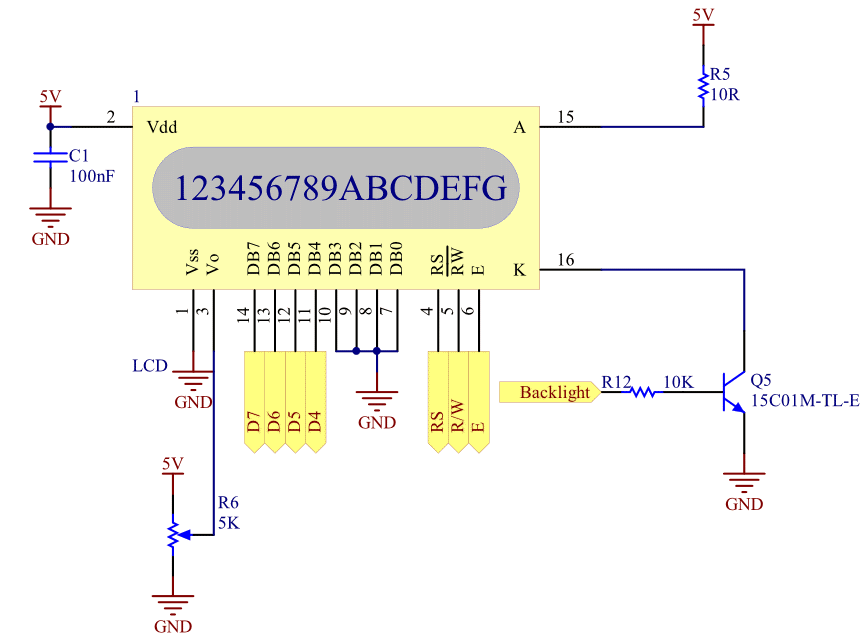
\includegraphics[width=100mm]{LCDSchematic.png}
	\rule{35em}{0.5pt}
	\caption[LCD Display Schematic]{Schematic of the LCD connections, showing the 4-bit LCD data bus mode and backlight driver transistor.}
	\label{fig:lcdschematic}
\end{figure}

\FloatBarrier
\subsubsection{Buttons}

A pair of standard PCB round buttons were added to the design, for user input. These buttons were wired directly to the microcontroller's GPIO pins; internal pull-up resistors in the microcontroller takes care of maintaining a defined logic level on the pins when the buttons are released, while software handles the debouncing of the button signals.

\FloatBarrier
\subsection{Headlights}

To provide illumination of the area immediately ahead of the robot, a pair of high intensity wide viewing angle white LEDs were added to the schematic, connected to a single common driver transistor and driven by a GPIO pin of the microcontroller. To ensure maximum illumination, the LEDs were driven at just under their full 20mA rating when turned on. These ``headlights'' were then mounted on the front of the robot chassis.

\FloatBarrier
\subsection{Speaker}

A small PCB Piezo speaker was added to the robot, in order to provide both audio feedback for important events (such as Bluetooth connections and disconnections) as well as to act as a miniature horn to attract the attention of any organic obstacles to encourage then to move away from the robot's line of motion. Rather than mounting the speaker directly onto the PCB, it was determined that a better location was in between the two frontal headlight LEDs, with the speaker then connected back to the PCB via flyleads. This arrangement made the directional speaker point in the orientation most suited to a car horn, i.e. towards the front of the robot (see Figure \ref{fig:robotspeaker}).

\begin{figure}[tbph]
	\centering
		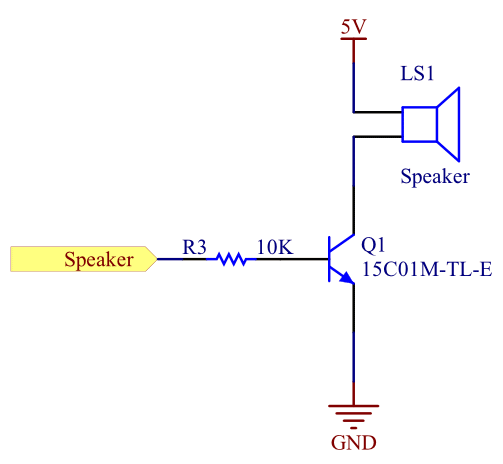
\includegraphics[width=55mm]{SpeakerSchematic.png}
		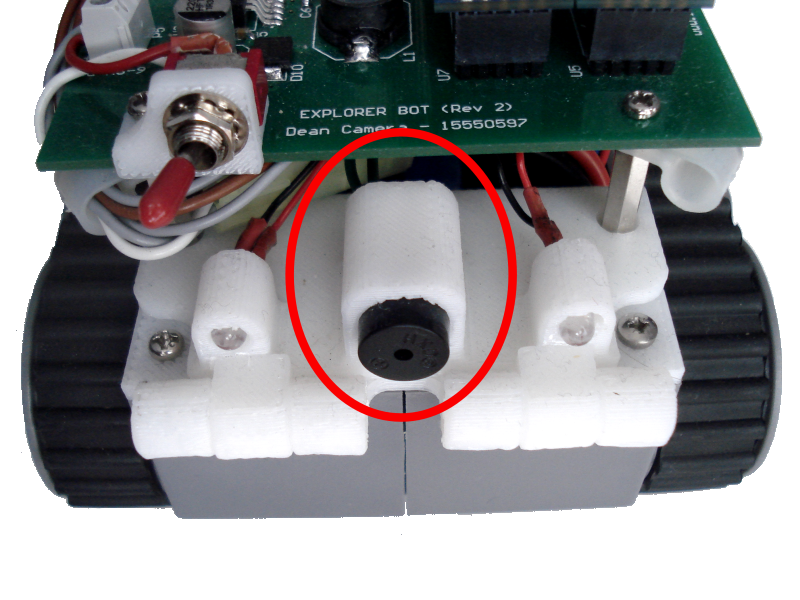
\includegraphics[width=60mm]{RobotFront.png}
	\rule{35em}{0.5pt}
	\caption[Speaker Schematic and Mounting Photo]{Schematic of the robot's piezo speaker (\textit{left}) and photo showing the mounting in the robot prototype (\textit{right}).}
	\label{fig:robotspeaker}
\end{figure}

To drive the speaker, a standard NPN transistor was employed to provide sufficient current, driven from an 8-bit PWM timer output GPIO pin of the AVR microcontroller.

\FloatBarrier
\subsection{Motor Controller}

While the plastic hobbyist ``tank'' style robot base selected for the prototype robot contained a pair of 6V DC motors stock from the factory, it did not contain a motor control system; implementation of a suitable motor control circuit was thus required as part of the project. To prevent motor noise from being injected back into the main 5V power supply used by the sensitive microcontroller, the motors were instead powered directly from the raw battery voltage. By directly powering the motors from the system battery, the main 5V logic power bus could remain relatively undisturbed by the potentially large current spikes caused by the switching on and off of the motors under load. This design had the additional benefit of a reduced the total power draw on the main power supply, reducing wasted power due to the supply's non-perfect efficiency and prolonging the operating time of the robot on a fresh battery.

As the raw battery voltage (7.2V nominal) was higher than the motor's 6V maximum, a PWM circuit was thus designed so that the average power delivered to each motor would prevent the motor from burning out during use. While not used in the final robot firmware, the use of variable duty cycle PWM drive signals to the motor would allow for additional speed control of the robot's motors without a corresponding loss of torque.

The motor controller design used in the project centered around the well-known conventional L298N Dual Channel Full H-Bridge Driver IC, notable for its high current drive capabilities and low-voltage logic level drive input support (see Figure \ref{fig:hbridge}). Originally the L298D variant was selected due to its convenient internal flyback diodes, however at the time of parts ordering a cheap source for the part could not be found. Unfortunately, the original PCB design did not allow for the possibility of adding external flyback diodes, resulting in the need for a second revised PCB manufacturing run to add in space for the missing components (see Figure \ref{fig:flybackdiodes}). Due to space constraints, the L298N's current sensing capabilities for motor stall detection were not used.

To correctly drive the L298N's PWM inputs, it was necessary to construct a logically inverted version of the PWM signal from the main microprocessor, which would be fed into the L298's channel compliment pin in order to correctly switch on and off the correct portions of the internal H-Bridge circuit. As the chosen microcontroller did not contain enough free pins for this function, an pair of external inverters were constructed out of discrete parts (see Figure \ref{fig:transistorinverter}). This basic logic inverter was used to invert each of the two motor PWM signals for the H-Bridge IC.

\begin{figure}[tbph]
	\centering
		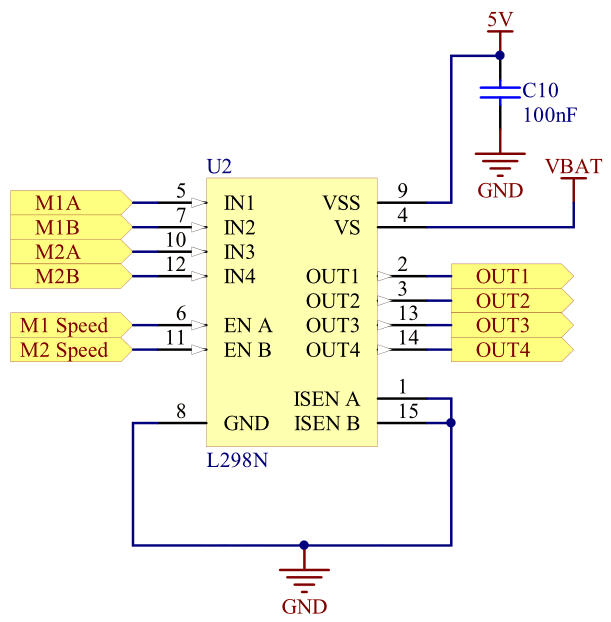
\includegraphics[width=55mm]{HBridgeSchematic.png}
	\rule{35em}{0.5pt}
	\caption[Motor H-Bridge Schematic]{Schematic of the L298N H-Bridge circuit used.}
	\label{fig:hbridge}
\end{figure}

\begin{figure}[tbph]
	\centering
		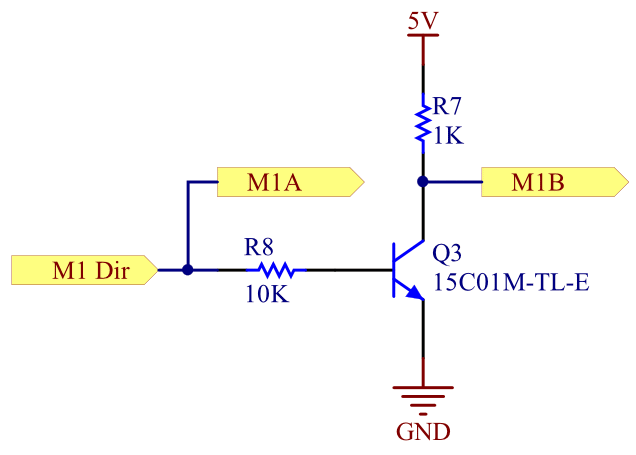
\includegraphics[width=55mm]{TransistorInverter.png}
	\rule{35em}{0.5pt}
	\caption[Transistor Inverter Schematic]{Schematic of one of the transistor inverters used to generate the compliment of the PWM signal used by the motor H-Bridge.}
	\label{fig:transistorinverter}
\end{figure}

\begin{figure}[tbph]
	\centering
		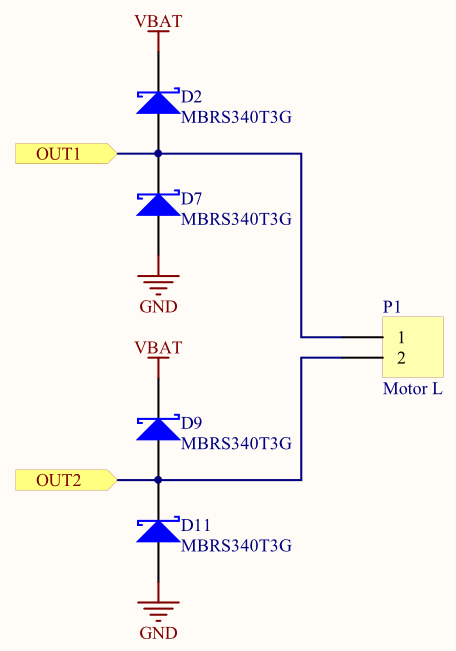
\includegraphics[width=55mm]{FlybackDiodeSchematic.png}
		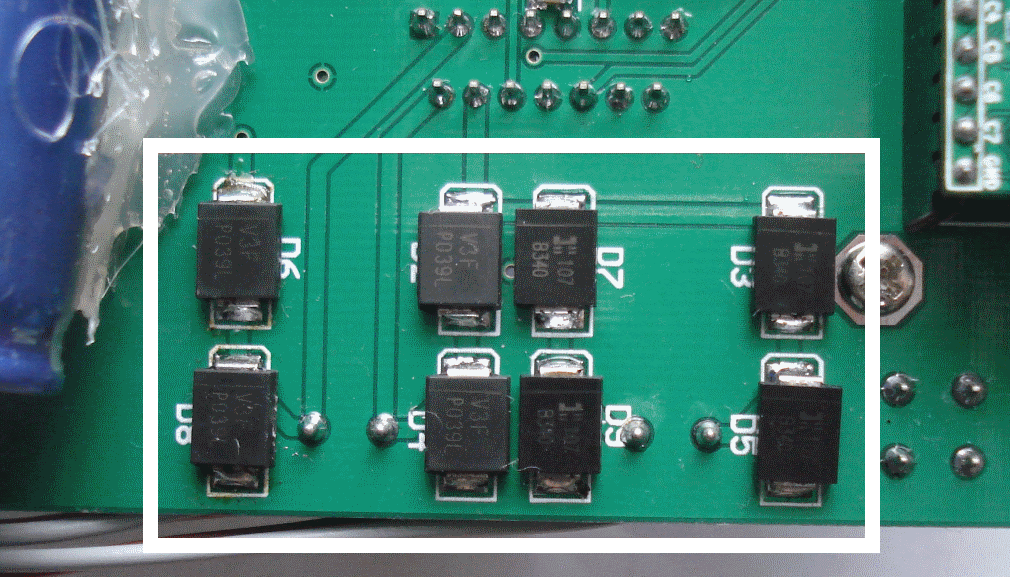
\includegraphics[width=80mm]{FlybackDiodes.png}
	\rule{35em}{0.5pt}
	\caption[Motor Flyback Diodes]{Partial schematic \textit{(left)} and photo \textit{(right)} of the external flyback diodes added in the second PCB revision to the robot's motors.}
	\label{fig:flybackdiodes}
\end{figure}

\FloatBarrier
\subsection{Sensors}

To provide a measure of feedback from the robot, a number of sensors were added to the design. These sensors, when attached, would allow for the robot's environment to be logged and (potentially) reacted to.

\FloatBarrier
\subsubsection{Sensor Power Supply}

While the main system logic and user interface components run from the main switch-mode 5V power supply, the sensor boards were required to run at a fixed 3.3V level, without the possibility of conversion to suit the higher rail voltage.

For this reason, and to reduce the amount of noise on the sensor power supply for maximum precision, a decision was made to add a secondary power supply, running from the 5V rail, to step down the voltage to the 3.3V required by the sensor boards. For best results, an ADP3308 Low Dropout (LDO) style regular was used as this provided both low output rail noise and minimal wasted power.

\FloatBarrier
\subsubsection{Level Converters}

Due to the differing bus voltages between the sensor boards (3.3V) and the main processor (5V), level conversion of the I\textsuperscript{2}C bus and sensor interrupt/control lines was required. While only a unidirectional buffer was strictly needed for each of the sensor interrupt/control lines, it was decided to use a bidirectional converter to ease the board routing.

Initially, only an ADG3308 8-channel Bidirectional Level Converter IC was used, for both the sensor interrupt/control lines, as well as the I\textsuperscript{2}C bus. However, after further analysis it was discovered that the level translator would not meet the timing requirements of the I\textsuperscript{2}C bus, necessitating the addition of a secondary dedicated Texas Instruments PCA9306 fixed function I\textsuperscript{2}C bus level converter IC in the second revision of the board. As a bonus, the use of the later chip allowed the I\textsuperscript{2}C bus to be driven at the ``Fast'' I\textsuperscript{2}C speed of 200KHz for minimal latency and maximum throughput.

Unusually, the ADG3308 level converter IC required that its enable pin (located on the low voltage side of the translator) be connected to the higher logic level for the chip to become active (see Figure \ref{fig:ADG3308schematic}). This odd placement of the enable pin resulted in a non-optimal breaking of the ground plane underneath the chip to accommodate the required route, as the space between the chip package pins on the top layer was used to carry the 3.3V power bus to the sensor boards (see Figure \ref{fig:ADG3308routing}).

\begin{figure}[tbph]
	\centering
		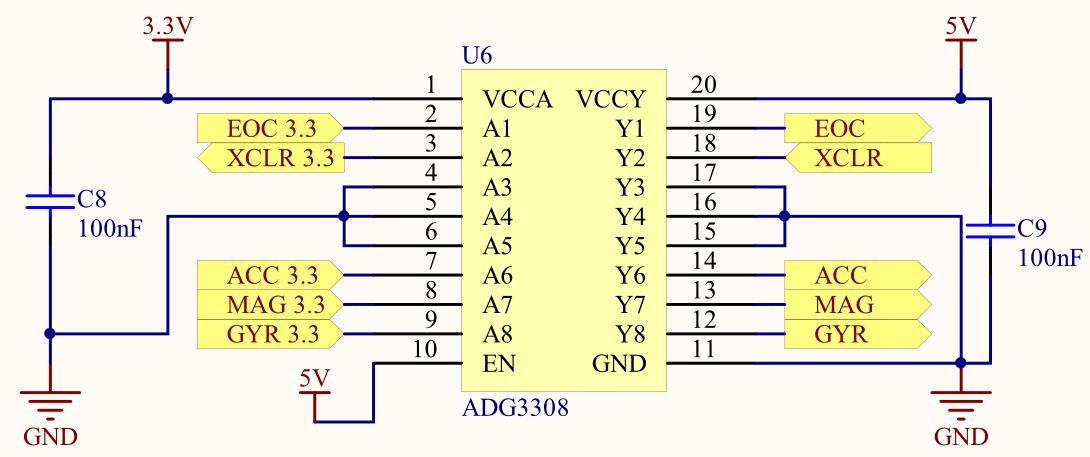
\includegraphics[width=120mm]{LevelTranslatorSchematic.png}
	\rule{35em}{0.5pt}
	\caption[Bidirectional Level Translator Schematic]{Schematic of the ADG3308, showing the unusual placement of the VCC-Y level active high enable pin.}
	\label{fig:ADG3308schematic}
\end{figure}

\begin{figure}[tbph]
	\centering
		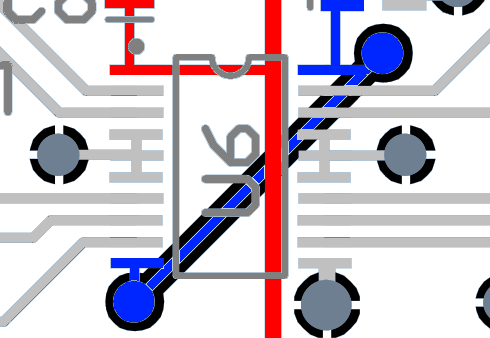
\includegraphics[width=50mm]{LevelConverterRouting.png}
	\rule{35em}{0.5pt}
	\caption[Bidirectional Level Translator Routing]{Routing of the ADG3308, showing the 3.3V bus (red) and 5V enable (blue) routes.}
	\label{fig:ADG3308routing}
\end{figure}

The board routing complexity was reduced slightly by swapping the functions of the PCA9306 bus level translator's SDA and SCL pins (see Figure \ref{fig:PCA9306schematic}) on both sides of the IC; this modification (allowable as indicated in the device's datasheet) prevented the need to introduce additional board vias and longer trace routes.

\begin{figure}[tbph]
	\centering
		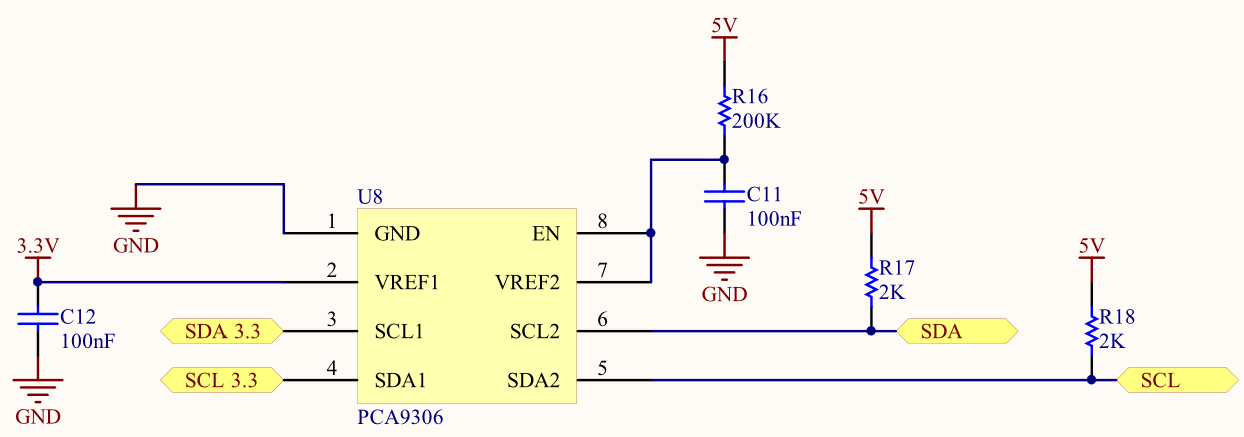
\includegraphics[width=140mm]{I2CTranslatorSchematic.png}
	\rule{35em}{0.5pt}
	\caption[I\textsuperscript{2}C Level Translator Schematic]{Schematic of the PCA9306, showing the swapped SDA and SCL pin functions.}
	\label{fig:PCA9306schematic}
\end{figure}

\FloatBarrier
\subsubsection{Atmel Sensor Boards}

By designing the robot around a pair of commercially available Atmel sensor boards for environmental feedback, the design of the robot was considerably simplified and the total unit cost lowered. The \textit{Atmel Pressure One} board contains a Bosch BMP085 Pressure Sensor IC for air pressure sensing, while the Atmel \textit{Inertial One} contains a 3-Axis ITG3200 Gyroscope, 3-Axis BMA150 Accelerometer and 3-Axis AK8975 Compass IC (see Figure \ref{fig:atmelsensorboards}). As several of the sensors also contain a digital temperature sensor in addition to the primary sensor (for calibration and stability feedback) this functionality was also used by the robot to measure the environmental temperature in real time.

Each sensor IC is driven by the main microcontroller of the robot over the level converted I\textsuperscript{2}C bus and one or more digital interrupt/control lines. The Atmel sensor board modules all use an identical form factor, with one standard .1" 2x5 female header located at one end of the board reserved for the mounted sensor's digital I/O pins, and another located at the opposite end of the board reserved for analogue sensor pinouts. As none of the sensor boards used contained analogue sensor outputs, the second female header consisted only of non-connected pins, and a matching male header was placed on the board for mechanical stability only.

\begin{figure}[tbph]
	\centering
		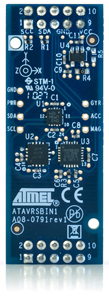
\includegraphics[height=70mm]{Inertial1.jpg}
		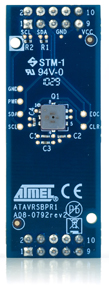
\includegraphics[height=70mm]{Pressure1.jpg}
	\rule{35em}{0.5pt}
	\caption[Atmel Sensor Boards]{The Atmel \emph{Inertial One} (left) and \emph{Pressure One} (right) Sensor Boards (Image courtesy \textit{Atmel Corporation})}
	\label{fig:atmelsensorboards}
\end{figure}

\FloatBarrier

	\chapter{Robot Firmware Implementation}
\label{chp:robotfwimp}
\lhead{Chapter \ref{chp:robotfwimp}. \emph{Robot Firmware Implementation}}

With the creation of the software embedded Bluetooth stack and the \textit{ExplorerBot} test robot platform hardware, it was necessary to integrate these two components into a functional prototype. By using the Bluetooth stack in a real-world, practical application while it was being developed, the quality, effectiveness and completeness of the stack could be evaluated.

\section{Build Dependencies}

To match the Bluetooth stack, each module was written in the C language, and targeted at the free open source AVR-GCC compiler and avr-libc library. A standard \textit{makefile} included with the firmware allows for command line control over the building of the project files into a set of binaries which can then be programmed into the target microcontroller for use via the command \texttt{make all}. The following tools are required to build the firmware under Windows:

\begin{itemize}
	\item The \textbf{WinAVR 20100101} release download, or Windows binaries of the \textbf{GNU Shell Utilities}
	\item The latest \textbf{AVR Toolchain} release from Atmel (Included with Atmel's free \textit{AVRStudio 5} software)
\end{itemize}

Under Debian Linux environments, the following packages are required:

\begin{itemize}
	\item \textbf{gcc-avr} 
	\item \textbf{binutils-avr}
	\item \textbf{avr-libc}
	\item \textbf{avrdude}
\end{itemize}

Which can be installed via the command prompt using the command \texttt{sudo apt-get install gcc-avr binutils-avr avr-libc avrdude}.

\section{Firmware Overview}

The completed firmware of the \textit{ExplorerBot} prototype was developed in a modular manner, to match the corresponding hardware components. This top-down methodology ensured that each portion of the firmware could be mocked up, tested and integrated as needed. Additionally, separating out the firmware components into logical modules gave the final firmware a level of flexibility which should allow for easy modification to suit any hardware changes made to those of the prototype. The completed set of modules (see Figure \ref{fig:robotblockfw}) served as the complete firmware for the robot.

\begin{figure}[H]
	\vspace{1em}
	\centering
		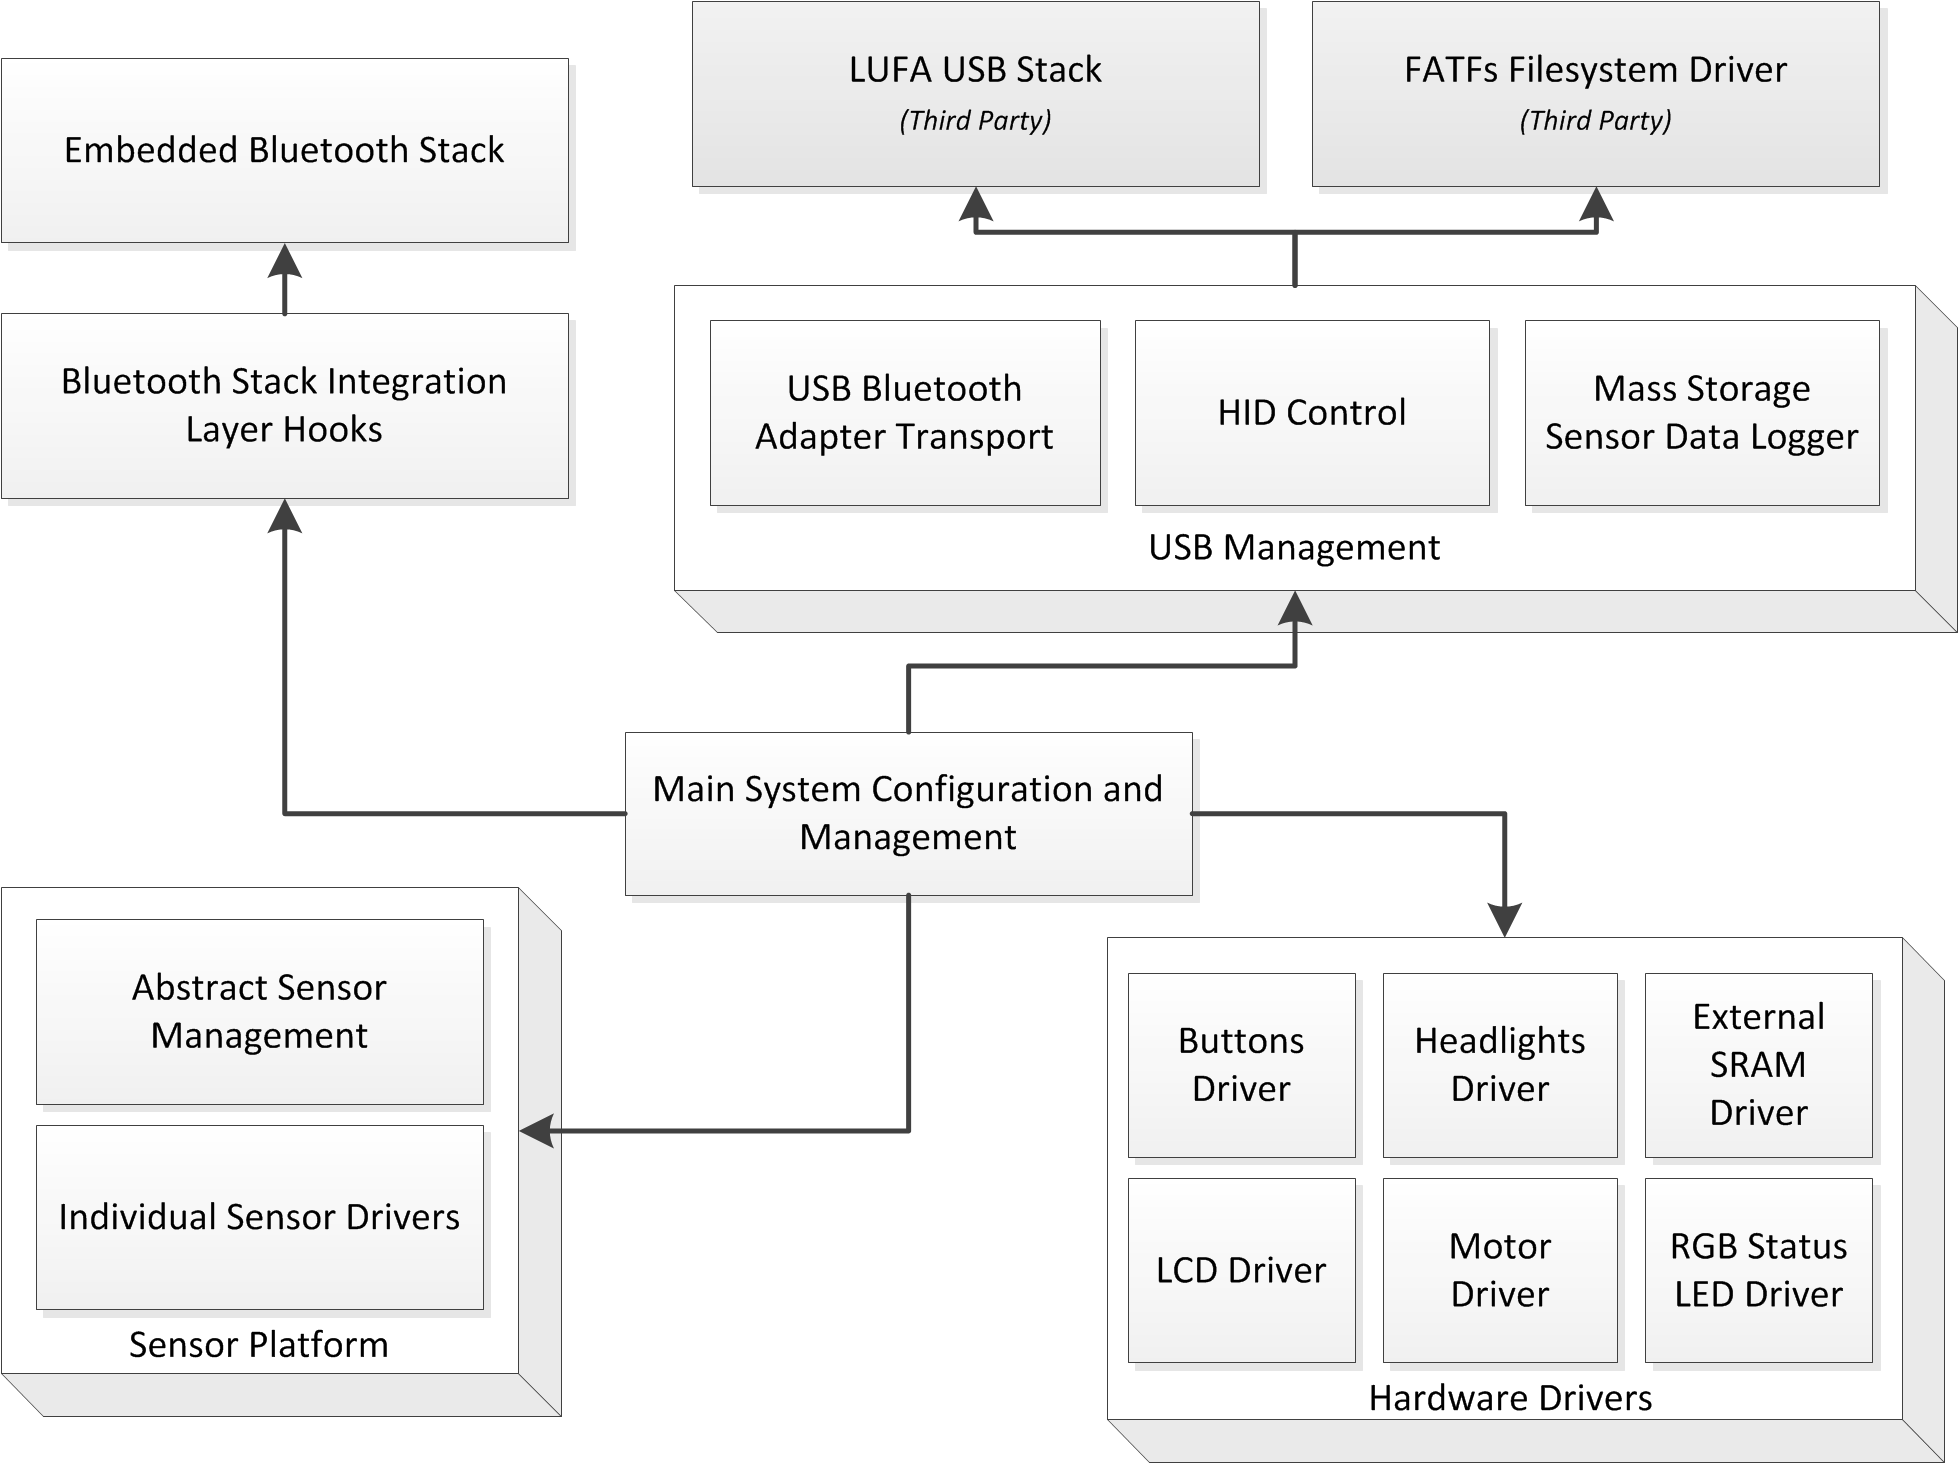
\includegraphics[width=140mm]{FirmwareBlockDiagram.png}
	\rule{35em}{0.5pt}
	\caption[Firmware Block Diagram]{Robot Firmware Block Diagram}
	\label{fig:robotblockfw}
\end{figure}

\section{Firmware Modules}

In this section, each of the robot firmware's main software modules are listed and described in additional detail so that the overall design and implementation of the firmware can be further understood.

\FloatBarrier
\subsection{Main System Control and Configuration}

The main entry point and system loop of the firmware was contained into a single top level module. This module was then made responsible for the initial system hardware configuration, as well as the management of the main loop to dispatch the service task functions in each sub-module.

\FloatBarrier
\subsubsection{System Initialization}

A series of initialization steps are followed during the hardware configuration step; first, the system watchdog (enabled if the chip was last reset through the expiry of the watchdog peripheral's timer) is disabled, the system CPU clock prescaler disabled to ensure the full 16MHz CPU clock speed is used, unused peripherals are powered down and the JTAG debug interface turned off so that the GPIO pins could be used for the RGB status LED. This latter procedure removes the ability to debug the firmware with an external JTAG debugger, however during development it was commented out.

Next, the setup routine calls each hardware driver module's \lstinline{Init()} function, which serves to initialize each hardware module and configure the appropriate hardware ready for use. Finally, one of the robot's remaining 16-bit hardware timers is then configured to run at a 10ms period to serve as the master system tick for timeout management and time based events.

\FloatBarrier
\subsubsection{Start-up Tasks}

Once all the system hardware is initialized, the main program flow then executes the start-up tasks; an informational message is displayed to the LCD while the RGB status LED sequences through all possible combinations, and the sensor platform is initialized to determine which sensors are currently connected. The state of each sensor is then displayed briefly onto the LCD using custom LCD character definitions before the main loop starts (see Figure \ref{fig:sensorinitlcd}).

\begin{figure}[tbph]
	\vspace{1em}
	\centering
		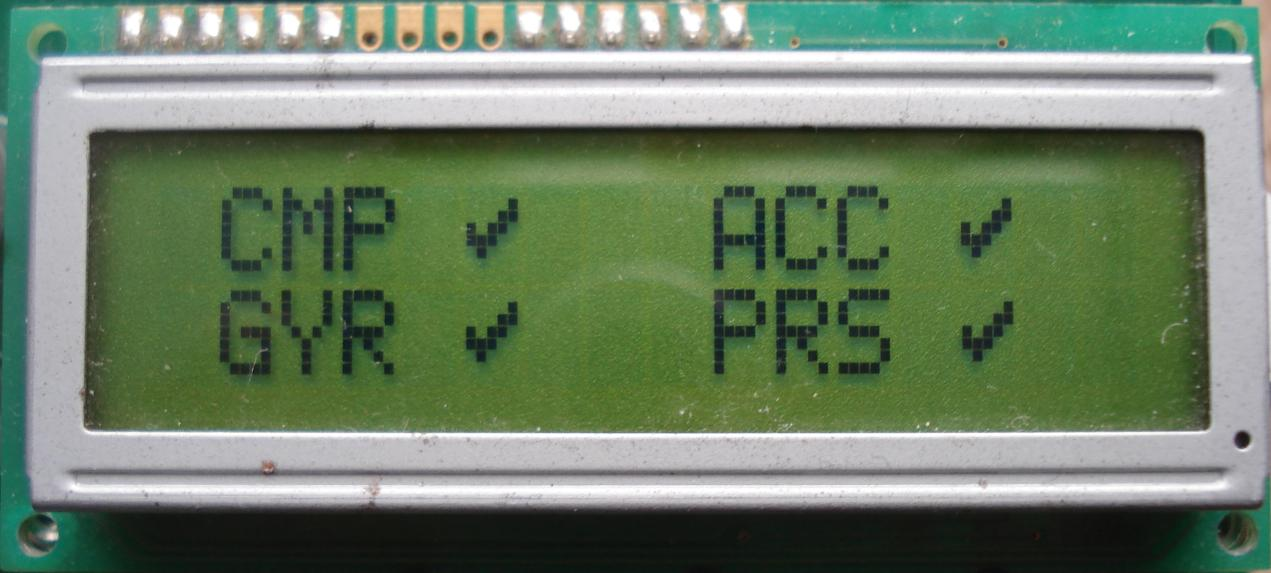
\includegraphics[width=70mm]{LCDSensorsOK.jpg}
		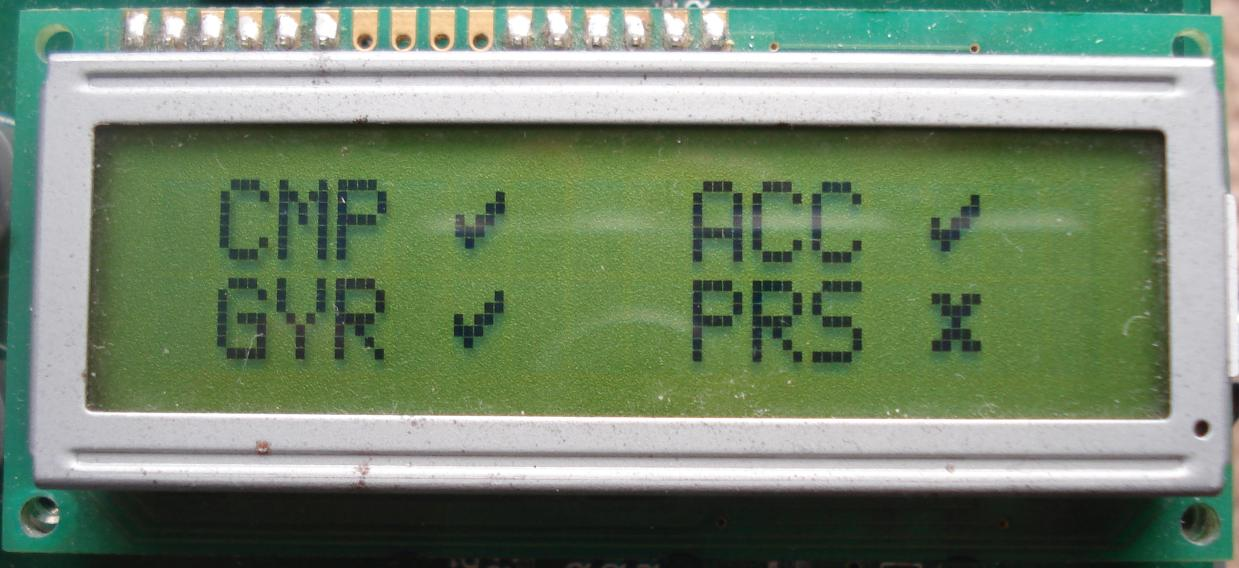
\includegraphics[width=70mm]{LCDSensorsFail.jpg}
	\rule{35em}{0.5pt}
	\caption[LCD Sensor Status Information]{Photos of the LCD display showing successful (\textit{left}) and failed (\textit{right}) initialization.}
	\label{fig:sensorinitlcd}
\end{figure}

\FloatBarrier
\subsubsection{Main Program Loop}

As is the case with virtually all embedded systems, the main program execution was contained in an infinite loop; each iteration of the loop would dispatch to the various sub-components of the system to manage and react to various stimuli. In the case of the robot firmware, the main loop contained three main functions; one, it checked for presses of either of the two physical buttons on the robot, two, it would check for expiry of the system tick timer to dispatch timing-related events, and three, it would execute the various hardware and software module service tasks.

In the case of the two physical buttons, the first (top) button was assigned a soft-reset role, in the case of a communication failure which resulted in the robot's motors being left on and the system uncontrollable. This \textit{emergency stop} style functionality was implemented using the microcontroller's internal watchdog system to reset the microcontroller approximately 15ms after the button press was detected. The second physical button was assigned a mode-specific role, according to Table \ref{tab:buttonroles}.

\begin{table}[tbph]
	\vspace{1em}
	\begin{center}
		\begin{tabular}{ | l | l | }
			\hline
			\textbf{Mode} & \textbf{Function} \\ \hline

			Bluetooth Mode & Initiates a connection to stored Bluetooth device address \\ \hline
			HID Mode & \textit{Unused} \\ \hline
			Mass Storage Mode & Enables sensor logging to the attached flash drive \\ \hline
		\end{tabular}
		\caption[Mode Specific Button Roles]{Table showing the function of the mode-specific physical pushbutton.}
		\label{tab:buttonroles}
	\end{center}
\end{table}

Each time the main loop detected that the system update tick timer period had elapsed, it would notify all timing-dependant hardware modules of this fact; for example, the LCD driver relies on these updates to automatically fade the LCD backlight brightness after a given period of inactivity. Also performed in this section is the update of the sensor values via the sensor platform at regular intervals, and the logging of this data either to the attached Mass Storage USB disk (if logging is enabled) or an established virtual serial connection to a remote PC via Bluetooth.

\FloatBarrier
\subsection{Hardware Drivers}

At the point at which the abstract software in the device needed to interact with the physical board hardware, a set of hardware abstraction drivers was created. These drivers served to encapsulate the functionality of the physical hardware and expose that functionality to the rest of the firmware via a set of basic control API functions. Not every driver sought to expose all the possible abilities of the hardware; due to time constraints only those features actually required by the prototype robot firmware were implemented in most cases.

\FloatBarrier
\subsubsection{Buttons Driver}

The hardware for the board button driver was, as expected, very simple; no debouncing was implemented in the driver itself, as this was not found to be necessary in the firmware. Adequate debouncing for the button logic could be achieved elsewhere in the code instead, via the software flags the buttons controlled.

As a result, the completed button driver implementation was trivial, consisting only of a configuration routine to configure the appropriate GPIO lines as inputs with the microcontroller's internal pull-up resistors enabled, and a status routine to read and mask out the appropriate port lines.

\FloatBarrier
\subsubsection{External SRAM Driver}

While the selected AT90USB1287 microcontroller contained 8KB of SRAM internally for stack, global variables and other working-set data, an external 128KB SRAM IC was mounted externally on the microcontroller board. This memory was attached to the AVR's external memory interface bus, and could then be used to extend the SRAM memory space at the cost of an extra CPU cycle for each external bus access.

Unfortunately, while this external SRAM memory uses a 17-bit address, the AVR's external memory bus interface is only 16-bits wide. As a result, a small software shim driver was required to perform manual bank swapping when required to select one of the two halves of memory. This total 128KB of external SRAM memory was thus divided into two 64KB memory banks, only one of which could be selected at one time.

\FloatBarrier
\subsubsection{Headlights Driver}

Like the button driver, the headlight driver contained only a thin wrapper around the GPIO pin used to control the robot's headlights. Latching of the headlight state was achieved through the GPIO hardware itself; once set to a particular state, the headlights would remain in that state (illuminated or disabled) until changed by a subsequent call to the module's update routine.

\FloatBarrier
\subsubsection{LCD Driver}

The LCD chosen for the robot contained a chipset compatible with the HD44780 display controller, common to many embedded systems where complex graphics are not required. As a result, there is already a plethora of LCD drivers available on the internet from hobbyists and from most microcontroller silicon vendors. Despite this, a simple custom LCD driver was written from scratch for the project, to ensure that as much of the project as was practical remained under the sole author's copyright and distribution control.

While the robot hardware contained a direct hardware connection to the LCD display's \textit{R/W} pin (for read/write control) the final driver code used a more basic hard-coded busy-wait delay method to ensure the display's timing was met. This practice proved to be the easiest to implement however for better performance this would have to be re-written as a polling scheme of the LCD controller's logical busy flag to reduce the system latency.

To conserve battery life, the LCD driver implemented an optional auto-dimming feature for the LCD backlight; when enabled, the display backlight would remain at full brightness after any updates for several seconds, before being faded gradually down to half brightness. This feature ensured that the display remained visible even in low-light conditions, but the reduction in brightness conserved battery power from the relatively power hungry backlight.

\FloatBarrier
\subsubsection{Motor Driver}

To drive the external H-Bridge circuit used in the robot's motor controller hardware, a software module had to be written to correctly generate the required direction and pulse train signals. A single 16-bit hardware timer was used for this purpose, with its dual PWM outputs connected to the motor control circuit hardware.

The function to control the motor output was significantly more complex than anticipated, due to the slow switching characteristics of the inverter hardware chosen (see Chapter \ref{chp:results}). The resulting driver had to ensure that during a direction change of one or more motors, the PWM signal of the motor would be completely disabled, to prevent momentary shorts of the main battery during the switching period.

Through trial and error, the motor PWM timer period was set to \lstinline{0x0FFF}, giving a frequency of around 8.1KHz at 16MHz due to the disabled prescaler and chosen \textit{``Phase Correct''} timer mode. Values below this range moved the PWM frequency noticibly into the range of human hearing, while raising this frequency reduced the efficiency of the motors and reduced the motor drive torque.

\FloatBarrier
\subsubsection{RGB LED Driver}

Like the robot headlights driver, the RGB status LED driver contained very little complexity. As a convenience, this driver exposed two sets of \lstinline{enum} values which could be used to set the colour of the RGB LED on the board. The first enum contained the literal colour names, which could be used to set a particular colour, while the second enum contained logical aliases of these colours for the various system states (see Listing \ref{lst:rgbenums}).

\lstinputlisting[float=tbph,caption={RGB LED Driver's colour enums.},label={lst:rgbenums}]{./Figures/RGBEnums.c}

Either of these two enum's values could be passed into the RGB LED driver's update routine, however in most cases the second (logical alias) versions were used to allow for easy modifications to the status colours at a later stage if desired.

\FloatBarrier
\subsubsection{Speaker Driver}

To drive the robot's small piezo speaker, an 8-bit hardware timer on the AVR microcontroller was used to generate an appropriate PWM square-wave of variable frequency to control the speaker driver transistor. Calling functions may supply either a raw timer count value to set the PWM frequency, or they may use the \lstinline{SPEAKER_HZ()} macro exposed by the module to convert a desired frequency into the closest timer count value.

A secondary feature of the speaker driver is the ability to play back one of several predefined sequences of notes, which are embedded into the firmware. These sequences are then used to play audible status indications on request from an external module. Note sequences are encoded as arrays of 16-bit unsigned values; the upper byte of which contains the PWM timer value to load into the timer, and the lower byte contains the number of system ticks the note should play for. As a convenience, the module-internal \lstinline{SPEAKER_NOTE()} macro performs the required encoding from a given note frequency and duration in milliseconds. A \lstinline{0x0000} zero entry terminates each note sequence.

\FloatBarrier
\subsection{Sensor Platform}

As the robot contained an (optional) set of physical environment sensors, a \textit{``Sensor Platform''} module was created to logically encapsulate all aspects of the sensors---from initialization and updates, to data formatting of the retrieved values---into a single package that could be integrated into the rest of the project easily, but also remain extendable enough that it could also be re-used in other future projects. The sensor platform is comprised of two software layers; the abstract sensor management layer, and the physical sensor drivers.

\FloatBarrier
\subsubsection{Abstract Sensor Management}

While the robot's auxiliary sensor boards (the Atmel \textit{Inertial One} and \textit{Pressure One}) contained several different sensor ICs with very different characteristics, the Sensor Platform module was designed to abstract these differences out from the rest of the firmware. This abstraction was achieved by providing a pair of simple initialization and update functions, and a consistent structure for the retrieved data from each sensor. An additional pair of functions were written to convert the retrieved sensor values into a Comma Separated Values (CSV) format. Using this method of encoding the data ensured that the retrieved data could be streamed out to one or more logical consumers in a standardized manner. Missing sensors (either not mounted or faulty) are automatically ignored by the sensor platform once the call to their initialization function has failed to complete.

Unfortunately, this abstraction led to one notable problem; as each sensor has a variety of configuration parameters which are specific to that particular device (or physical property it measures) an abstract interface for sensor configuration could not easily be written. While this could be solved with additional design and planning, for the purposes of the project each sensor's configuration was instead fixed to sane defaults inside the physical sensor drivers, and no interface provided to alter these parameters on the fly externally.

The C language structure used to encapsulate the state of a single sensor is shown in Listing \ref{lst:sensorentry}. This structure definition is instantiated as an array inside the sensor platform, with one entry then being dedicated to each physical property being measured (as distinct from each physical sensor IC). In the case of the ITG3200 Gyroscope sensor IC, the internal temperature sensor was used in addition to the orientation data. In this particular case, the temperature sensor was assigned a second sensor structure entry in the sensor structure array.

\lstinputlisting[float=tbph,caption={Sensor Platform's Abstract Sensor entry structure definition.},label={lst:sensorentry}]{./Figures/SensorPlatformEntry.c}

Of note is the use of a C \textit{union} to contain the retrieved sensor data, as either a single \lstinline{int32_t} signed 32-bit integer value, or a triplicate of three \lstinline{int16_t} signed 16-bit integers. The use of this union minimises the amount of memory used by each sensor entry, as the two mutually exclusive styles of returned data can overlap physically in RAM (see Figure \ref{fig:sensorentry}). For sensors returning only a single 32-bit value, the sensor initialization function sets the corresponding \lstinline{SingleAxis} item in the structure so that the platform knows how to extract and format the retrieved data.

\begin{figure}[tbph]
	\vspace{1em}
	\centering
		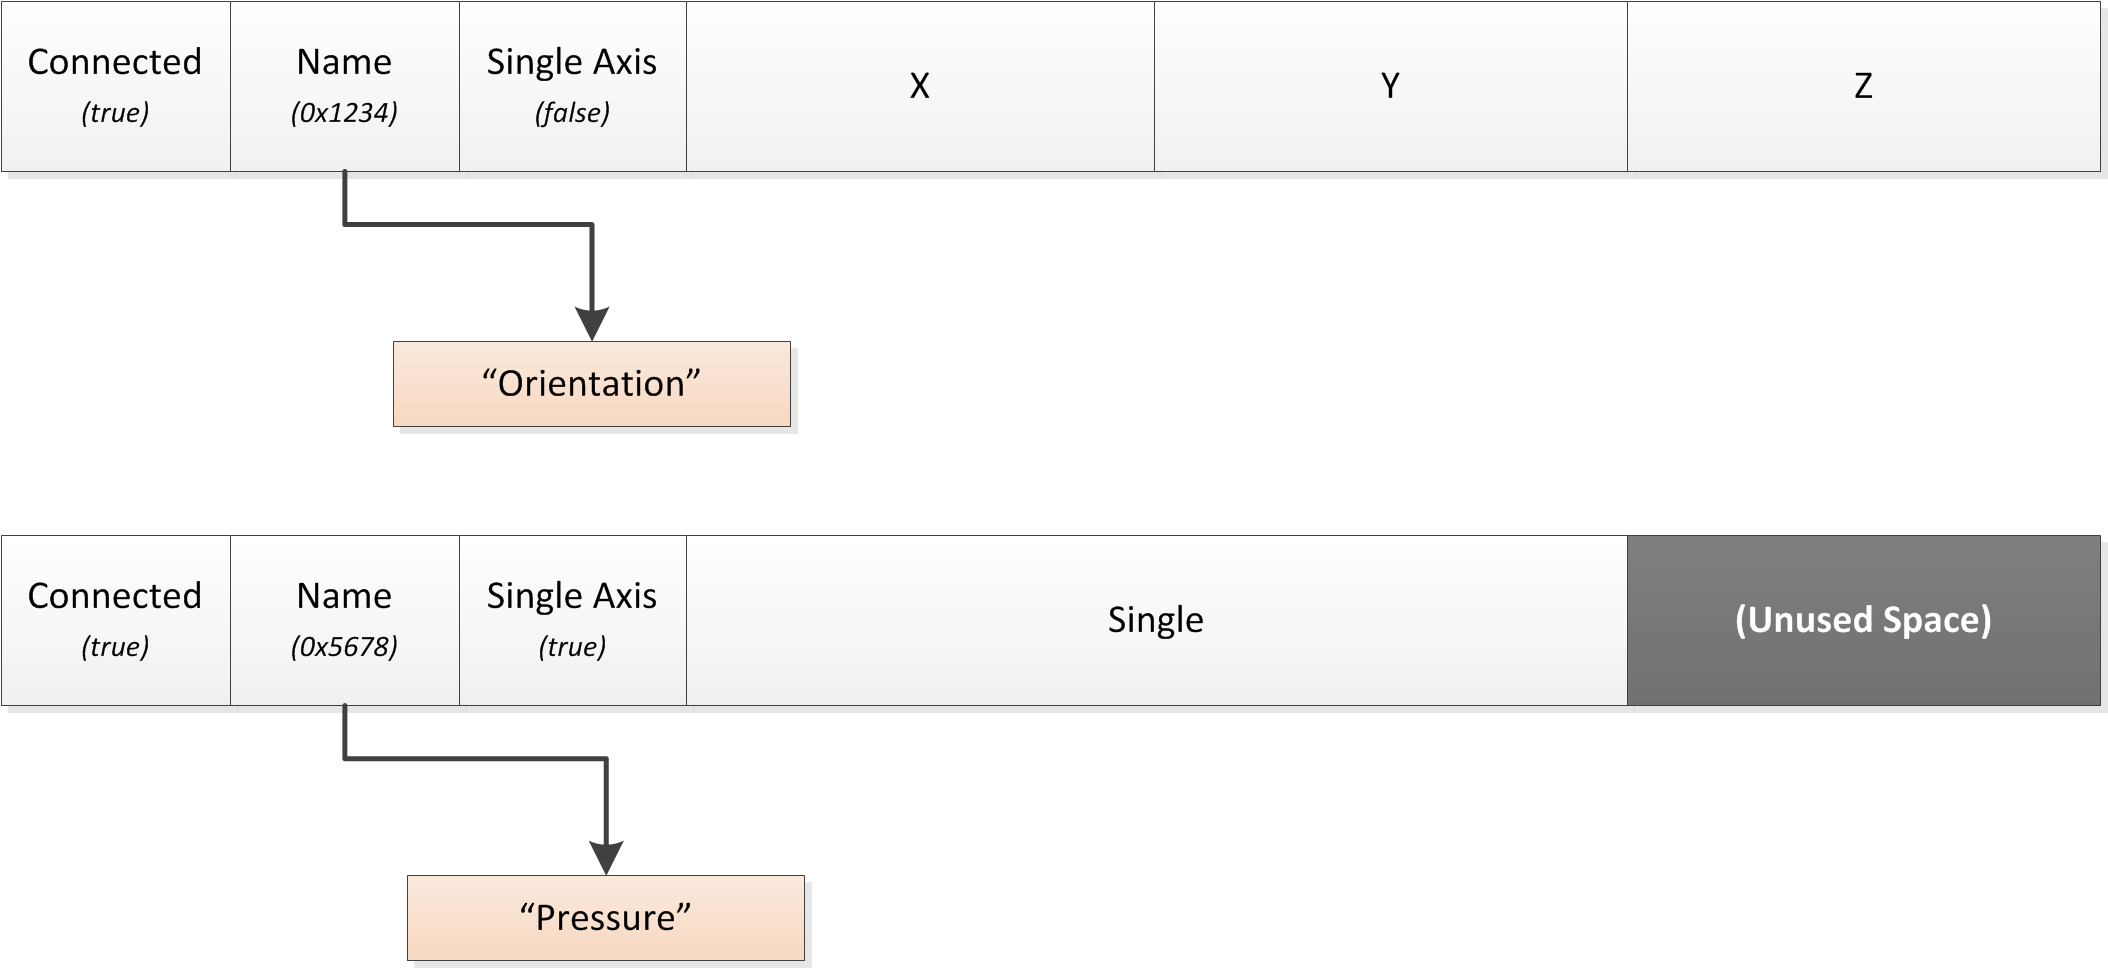
\includegraphics[width=130mm]{SensorPlatformEntry.png}
	\rule{35em}{0.5pt}
	\caption[Sensor Platform Entry Structure Diagram]{Diagram showing the layout of the Sensor Platform Entry structure in memory for triple axis (\textit{top}) and single axis (\textit{bottom}) sensors.}
	\label{fig:sensorentry}
\end{figure}

\FloatBarrier
\subsubsection{Individual Sensor Drivers}

Each individual sensor connected to the board requires a custom sensor driver, specific to that make and model of sensor IC. Unique to each sensor is the sequence required to set up the sensor to a known set of default configuration parameters (see Table \ref{tab:sensorconfig}), as well as the exact command set, address of the I\superscript{2}C bus, and optional use of control/interrupt GPIO lines used in the sensor's operation.

\begin{table}[tbph]
	\vspace{1em}
	\begin{center}
		\begin{tabular}{ | l | l | l | l | }
			\hline
			\textbf{Sensor}	& \textbf{Type}	& \textbf{I\superscript{2}C Address} & \textbf{Settings} \\ \hline

			AK8975 & Direction & 0x0C & N/A \\ \hline
			BMA150 & Acceleration & 0x38 & \vtop{\hbox{\strut 25Hz bandwidth,} \hbox{\strut +/-2g range,} \hbox{\strut Interrupt line enabled}} \\ \hline
			BMP085 & Pressure & 0x77 & N/A \\ \hline
			ITG3200 & Orientation & 0x68 & \vtop{\hbox{\strut 100Hz at an internal sampling rate of 1KHz, } \hbox{\strut Low Pass Filter to use 20Hz bandwidth,} \hbox{\strut Gyroscope X axis PLL as the clock source,} \hbox{\strut Interrupt line enabled}} \\ \hline
			ITG3200 & Temperature & 0x68 & N/A \textit{(Virtual Sensor)} \\ \hline
		\end{tabular}
		\caption[Sensor Configuration]{Table showing the sensors used and their configuration properties.}
		\label{tab:sensorconfig}
	\end{center}
\end{table}

To ensure the interface into each individual sensor driver was as uniform as possible, the exact implementation details was hidden from external modules, with each driver exposing just two functions; an \lstinline{Init()} function to initialize the sensor, and an \lstinline{Update()} function to pull the latest values from the sensor if it has completed a conversion. To prevent slow sensors from introducing unnecessary lag into the system, the update functions would abort if the next conversion was not ready at the point in time that the function was called, and the sensor entry structure would retain the previously retrieved sensor value. Each time a completed sensor data conversion was read from the sensor, a new conversion was started asynchronously.

\FloatBarrier
\subsection{Third Party Modules}

While every effort was made to ensure that as much code as possible for the project was written from scratch, some allowances had to be made for third party libraries. Such libraries were used in places where the complexity of the module would hinder the project if a new implementation had to be implemented from scratch within the project's timeframe.

\FloatBarrier
\subsubsection{LUFA}

A crucial part of the project was the ability to communicate with USB devices; the AVR's USB interface was to be used for both configuration and control of the robot, via a variety of USB devices. A full USB stack is a rather complicated affair; generally it takes an entire team of programmers working together and ample debugging time to produce a functional stack. Because of the short timeframe of the project, an existing stack was chosen instead.

The selected stack was LUFA, the \textit{Lightweight USB Framework for AVR devices}. This stack, a personal side-project of the author, offers a rich device support in both USB host and device modes. The library contains many inbuilt drivers for the various classes of USB devices, some of which were used in the project for the HID joystick control and Mass Storage configuration and sensor logging.

For the robot firmware, LUFA version 20111009 was used.

\FloatBarrier
\subsubsection{FatFS}

To read and write files onto an attached Mass Storage USB device, it was neccesary to add a filesystem driver into the system. Using a standard filesystem allowed the firmware to maintain compatibility with files stored onto the disk using other devices. As the de-facto standard for embedded system filesystem is Microsoft's FAT (due to its relative simplicity when compared to more modern filesystems) a FAT compatible filesystem driver was selected for the project.

The third-party FATFs library was chosen for this task, as it offers a free, tested, portable and light-weight C implementation of the FAT filesystem standard. The FATFs library is compatible with most variants of the FAT standard (including FAT16 and FAT32) making it an ideal choice for the project. Linking the FATFs library's read and write callback functions to the LUFA USB library's Mass Storage class driver section functions proved to be much easier than anticipated (see Listing \ref{lst:fatfsshim}).

\lstinputlisting[float=tbph,caption={FATFs shim layer, connecting it to the LUFA USB Stack Mass Storage class driver.},label={lst:fatfsshim}]{./Figures/FATFsShim.c}

\FloatBarrier
\subsection{USB Management}

In order to support the various types of USB devices needed by the robot firmware, a collection of USB class-specific management layers were written. These layers, sitting in parallel on top of the LUFA USB stack, provide the routines neccesary to manage each type of supported USB device.

While the LUFA USB stack provides support for several of these classes of USB devices internally, additional code was required to wrap the existing USB class driver, to extend the provided functionality and interface the driver with the rest of the system.

\FloatBarrier
\subsubsection{Bluetooth Adapters}

The LUFA stack version used in the project did not contain a ready-made internal driver for USB Bluetooth adapters. A suitable driver was thus created specifically for the project using the USB transport specification outlined in the Bluetooth 2.1 specification document. In order to support all possible Bluetooth adapters from all silicon vendors, the driver was written to match generically on the defined \texttt{class}, \texttt{subclass} and \texttt{protocol} Device Descriptor values of \texttt{0xE0}, \texttt{0x01} and \texttt{0x01} respectively, as set by the Bluetooth specification for conformant Bluetooth adapters. By matching against these values instead of a particular Vendor ID and Product ID, the driver was able to support all devices conforming to the Bluetooth standard's USB transport interface specification without additional modifications being required.

During the enumeration process of an inserted USB device, the main function calls the module's \lstinline{BluetoothAdapter_ConfigurePipes()} function to attempt to bind it to the inserted USB device. The module first validates the device descriptor to ensure the inserted device is reportedly a Bluetooth adapter. Next, the pipe configuration routine attempts to configure the USB controller's logical data pipes so that the \textit{Data In}, \textit{Data Out} and \textit{Event In} pipes are correctly connected to their matching logical endpoints within the adapter. If the driver is unable to bind to the device for any reason, the enumeration process is aborted for the Bluetooth transport driver.

Periodically, the main firmware loop will call the Bluetooth transport driver's \\ \lstinline{BluetoothAdapter_USBTask()} service task if the transport driver is currently active. This service task is responsible for checking the logical data pipes for new data, and (if data is availiable) reading in the data packet before dispatching it to the Bluetooth stack. A \lstinline{CALLBACK_Bluetooth_SendPacket()} callback function from the Bluetooth stack takes care of sending packets generated from the Bluetooth stack to the Bluetooth adapter.

\FloatBarrier
\subsubsection{HID Devices}

For local diagnostics of the system before the Bluetooth stack was completed, a local Human Interface Device (HID) driver was implemented into the firmware. This driver builds on top of the HID class driver included in the LUFA distribution used, and binds supported HID devices (such as game controllers) to the robot's physical functions. Using this driver, a USB joystick or game controller can be inserted into the robot and used to control the motors, headlights and horn.

As most HID devices carry a unique physical and logical report layout, it is important to include a mechanism to correctly bind the appropriate buttons on the attached device to the correct logical function. Two seemingly identical USB joysticks can output very different report data structures to the host, requiring the use of a \textit{HID Descriptor Report Parser} to correctly parse the reports into a standard format. The HID Report Parser included in the LUFA USB stack was used for this purpose, and linked into the rest of the system. This allows the robot to maintain compatibility with virtually all HID devices containing an appropriate number of buttons.

\FloatBarrier
\subsubsection{Mass Storage Devices}

As a means of system configuration and monitoring, a Mass Storage Device (MSD) driver was also added into the device firmware. This proved useful for both fault-finding and data logging, as data produced by the firmware could be stored onto an inserted USB flash drive. During the initial firmware development, this functionality was used to store logs of the on-board sensor outputs, to ensure the correctness of the sensor platform before the completion of the wireless serial port functionality. At a later stage, this mode was extended so that it could be used to configure the target remote Bluetooth Devive Address used in the robot's Bluetooth Mode when a remote connection was initiated by the user.

To be able to read and write files on an attached USB flash disk drive, the FATFs library was linked to the LUFA Mass Storage class driver. This abstracted out the physical medium, giving a higher level file-centric view of the attached storage medium, as opposed to the direct physical sectors.

When a disk is inserted, the firmware will first attempt to open an existing file called \texttt{SENSLOG.CSV} on the disk, for sensor logging in CSV format (see Listing \ref{lst:logfileparse}). If such a file does not exist, a new one is created and the sensor log header (constructed by the Sensor Platform module) is written to the start of the new file.

\lstinputlisting[float=tbph,caption={Example of the Mass Storage manager code to open and write to a file on an attached USB flash disk using the FATFs library.},label={lst:logfileparse}]{./Figures/LogFileParsing.c}

Additionally, the firware will attempt to open and process a second file names \texttt{REMADDR.TXT}, which holds the Bluetooth device address of the remote Bluetooth device the robot should attempt a connection to upon demand. This file is expected to contain an address of the format \texttt{XX:XX:XX:XX:XX:XX}, containing the six consecutive octets of the remote device's address, in hexadecimal format. This address is then stored into the robot's non-volatile EEPROM memory for later use when a Bluetooth adapter is subsequently inserted. If no such file exists on the attached disk, one is created and the currently stored remote device address written to it.

\FloatBarrier
\subsection{Bluetooth Management Layer}

Connecting the project's Bluetooth Stack to the rest of the robot firmware was the Bluetooth Management layer, responsible for providing the appropriate callback function implementations required by the stack. These callback functions are fired by the Bluetooth stack in response to defined events, such as connection requests, channel establishment and packet reception.

A secondary duty performed by the management software layer is the dispatch of events and data to and from the various Bluetooth services. These services, such as RFCOMM, SDP and HID, are optional in all implementations, and thus require manual integration into each project on top of the base Bluetooth stack if desired. These services must be linked to the various Bluetooth stack callback events so that they may function correctly (see Listing \ref{lst:btdatacallback}).

\lstinputlisting[float=tbph,caption={One callback from the Bluetooth Stack, dispatching received packets to the integrated Bluetooth services.},label={lst:btdatacallback}]{./Figures/BTStackDataCallback.c}

In some cases, a Bluetooth enabled application may peform specific filtering on incoming connection and channel requests; an embedded device may be programmed to reject all but one specfic remote device, or only accept specific channel protocols. However, as the \textit{ExplorerBot} was designed to be controlled publically via any supported Bluetooth enabled device, no such filtering was performed in the request callback routines. All HCI connection and L2CAP channel event callbacks were implemented, however, to display their relevant event data onto the robot's LCD display for debugging purposes.

Inside this management layer, the RFCOMM service channel open and close events were hooked, so that the opened RFCOMM channel handles could be captured. This captured handle is then stored temporarily by the robot firmware and used for later streaming of the sensor data. As only one connection handle is stored by the device at any one time for this purpose, a limitation of the system is imposed; only one wireless serial port can receive sensor data at the one time.

The HID service callback for packet reception was also hooked in this layer, and implemented to process incoming HID reports from Bluetooth devices. These processed reports---from game controllers, mobile phones, or other HID compliant devices---were then fed back into the main firmware module to control the robot's motors, headlights and horn hardware.
	\chapter{Project Results}
\label{chp:results}
\lhead{Chapter \ref{chp:results}. \emph{Project Results}}

In this section, the results obtained and testing procedures used in the verification of the robot are detailed.

\section{System Testing}

An important part of any project is an appropriate level of testing, performed at both the hardware and software levels. Without adequate testing, undiagnosed latent issues such as hardware faults and software bugs may cause incorrect system operation. By performing at least some level of system testing, issues can be found and corrected as early as possible within the project's development process.

\FloatBarrier
\subsection{Board Level Testing}

During and after the construction phase of the robot's hardware, a number of verification tests were made to ensure that the various hardware modules were operating as expected. This step was critical in ensuring the correctness of the hardware before the main firmware was written, to rule out hardware errors in the software verification phase.

\FloatBarrier
\subsubsection{Main Power Supply}

The main power supply was tested with an oscilloscope, after the module components were installed onto the PCB. A static load of 300mA was placed on the switchmode supply output, and the voltage ripple on the supply measured with an oscilloscope (see Figure \ref{fig:mainpowerripple}). This yielded an output ripple of approximately 80mV, well within the tolerances of the system. At the given static load, the regulated output voltage was measured at 4.98V, within the specifications of \(4.8V\leq\text{V\subscript{out}}\leq5.2V\) listed in the LM2595-5 regulator datasheet.

\begin{figure}[tbph]
	\vspace{1em}
	\centering
		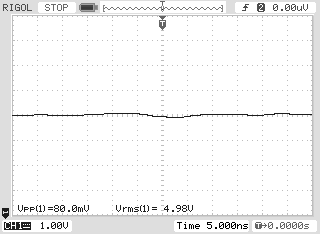
\includegraphics[width=90mm]{SM5V.png}
	\rule{35em}{0.5pt}
	\caption[Switch-mode 5V Power Supply Oscilloscope Trace]{Oscilloscope trace of the main 5V switchmode power supply showing ripple under static load.}
	\label{fig:mainpowerripple}
\end{figure}

\FloatBarrier
\subsubsection{Sensor Power Supply}

For the secondary 3.3V LDO power supply used by the board's sensor modules, an identical set of tests to those used in the verification of the main power supply were performed, using the sensor boards as the regulator output load. This yielded a ripple of 120mV, and an output voltage of 3.27V. When compared to the ADP3308 datasheet output's electrical characteristics, this was within the stated \(\pm1.2\%\) accuracy (\(3.26V\leq\text{V\subscript{out}}\leq3.34V\)).

\begin{figure}[tbph]
	\vspace{1em}
	\centering
		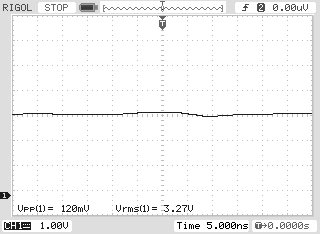
\includegraphics[width=90mm]{LDO3V.png}
	\rule{35em}{0.5pt}
	\caption[LDO 3.3V Power Supply Oscilloscope Trace]{Oscilloscope trace of the sensor 3.3V LDO power supply showing ripple under static load.}
	\label{fig:sensorpowerripple}
\end{figure}

\FloatBarrier
\subsubsection{Motor PWM Outputs}

To test the motor outputs (and, in turn, the entire motor controller circuit) the two motor output channels were connected to an oscilloscope in sequence, and a small test wrapper written over the motor driver firmware module. Each output was switched backwards and forwards at the maximum (safe) PWM rate, and the resulting waveforms verified against the expected waveforms. Figure \ref{fig:motorpwm} shows one such waveform, showing the left motor output at full speed.

\begin{figure}[tbph]
	\vspace{1em}
	\centering
		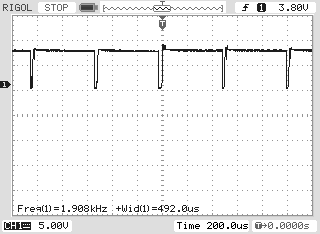
\includegraphics[width=90mm]{PWM.png}
	\rule{35em}{0.5pt}
	\caption[Motor PWM Oscilloscope Trace]{Oscilloscope trace of one motor channel PWM output while active, showing the frequency and duty cycle at full speed.}
	\label{fig:motorpwm}
\end{figure}

\FloatBarrier
\subsubsection{RGB Status LED}

A simple test routine was written to cycle through all possible colours on the mounted RGB status LED; this demonstrated that the three GPIO channels were configured and connected correctly, and that the appropriate brightness balancing for each sub-component in the LED package was set correctly by the chosen current limiting resistors on the board. As this is a simple but visually attractive piece of self-diagnostics, the test routine code was eventually retained in the final robot version during the robot's start-up sequence.

\FloatBarrier
\subsubsection{LCD and Backlight}

To test the board's LCD functions, a routine calling various formatting commands was written and wrapped around the completed LCD driver software module. These commands---containing various cursor placements, custom character definitions and formatted strings---indicated that the display was indeed working as expected. For the LCD backlight, code was written to slowly fade in the backlight brightness from the minimum value, up to the maximum in 10ms increments. Like the RGB LED test routine, this functionality was eventually incorporated into the start-up routine of the final robot firmware.

\FloatBarrier
\subsection{Software Testing}

At the conclusion of the hardware testing, a new set of software tests were performed on the robot firmware to ensure correct operation and compatibility with the appropriate specifications. This presented its own unique set of challenges, as suitable testing environments and testing procedures had to be developed.

\FloatBarrier
\subsubsection{USB Integration}

Small software tests were performed for the three supported USB classes; HID, Mass Storage and Bluetooth Adapters. Doubling as a test of the hardware drivers, the HID management driver was tested against a PS3 Controller and two generic HID class USB gaming controllers, to ensure that the appropriate buttons were mapped to the robot's functions. During these tests, a brown-out failure condition was observed on the USB bus when the robot's motors were switched on and off (or changed in direction) rapidly. This issue was traced back to the original ``AA'' cell bank battery's instantaneous current capabilities, and was temporarily corrected in the robot prototype with a large value capacitor on the battery input terminals (see Figure \ref{fig:mainpowercap}) until the more powerful Lithium-Ion battery pack was substituted.

\begin{figure}[tbph]
	\vspace{1em}
	\centering
		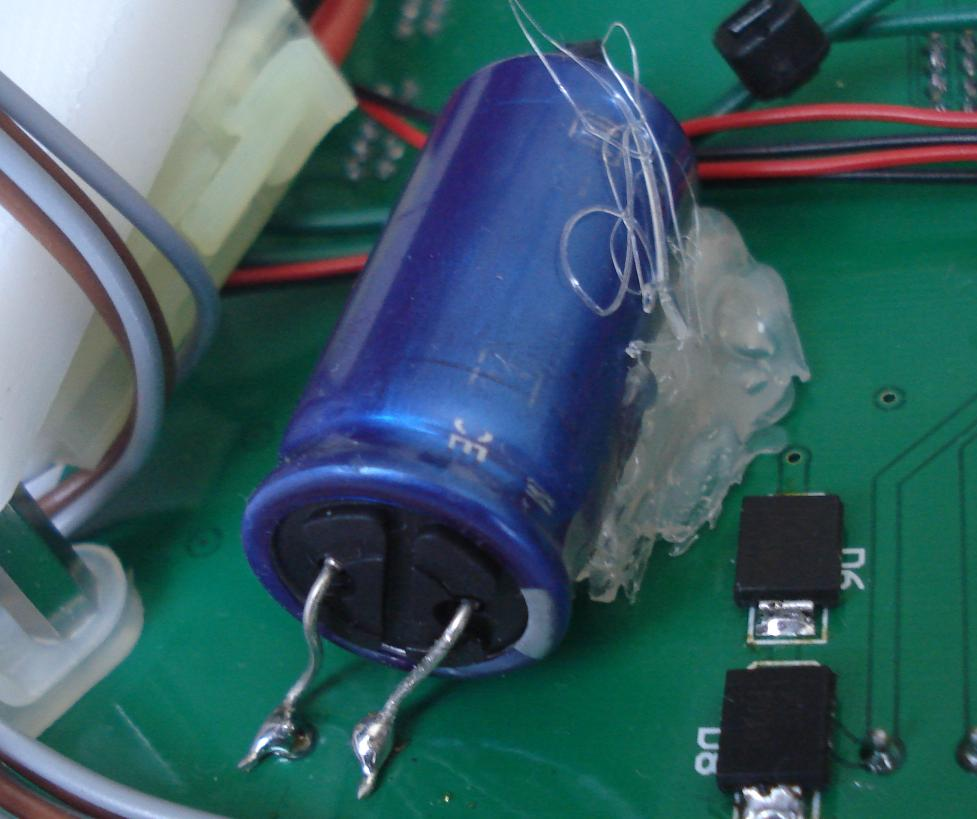
\includegraphics[width=60mm]{PowerCap.jpg}
	\rule{35em}{0.5pt}
	\caption[Temporary Main Power Input Capacitor]{Photo of the temporary main input power capacitor, to prevent brown-out conditions from motor-induced current spikes.}
	\label{fig:mainpowercap}
\end{figure}

The Mass Storage management module (and, by extension, the FATFs library it depends upon) was tested through a procedure of disk insertion and removal, with files written to and read from the disk filesystem using dummy data. Thus verified, the complete Mass Storage management file parsing routines were checked by printing the parsed file output to the robot's LCD display.

As the Bluetooth Adapter management code relied upon the upper Bluetooth Stack logical layers for correct operation, the functionality of the USB transceiver device management could not be examined and verified until the base layers on the Bluetooth Stack were completed. However, in this phase of the software testing, the module's ability to correctly bind to compatible Bluetooth devices in a generic manner (using several adapters from different manufacturers) was tested and found to function as expected.

\FloatBarrier
\subsubsection{Sensor Platform}

The sensor platform required a significant amount of time to complete and verify; the final development time was close to one and a half weeks, much more than the expected two or three days. A number of flaws were found in the written code when it was tested on the physical robot hardware, including a bug in the LUFA USB stack's I\superscript{2}C driver for packet read and writes. Timing and other issues in the written driver for the Bosch BMA150 accelerometer resulted first in no sensor output, followed by output on only one channel. The root cause of this problem was eventually tracked down to misleading datasheets, where the sensor would react correctly only if certain configuration registers were altered in specific manners to what should have been---according to the values given in the datasheet---the sensor's initial power-on defaults.

During the sensor platform testing phase additional small errors relating to the formatting and endianness of the retrieved values were also identified and corrected.

\FloatBarrier
\subsubsection{Bluetooth Stack}

The completed Bluetooth stack was tested in an iterative manner; as additional features and layers were completed, they were verified against existing third-party Bluetooth devices. An invaluable tool used in the verification and debugging of each layer and protocol was the Linux ``Bluez'' Bluetooth stack's \texttt{hcidump} tool, which allowed the robot's Bluetooth stack packets to be captured in real time and decoded, indicating any issues in the implementation of one or more protocols used in the device.

Listing \ref{lst:hcidump} shows a fragment of a HCI layer packet capture between a virtualized Linux environment and the robot, while successfully establishing a new L2CAP channel between the two devices for SDP discovery.

\lstinputlisting[float=tbph,caption={HCI packet capture during a L2CAP channel configuration.},label={lst:hcidump},language={bash}]{./Figures/HCIDump.txt}

The RFCOMM layer was examined and verified at both the L2CAP layer and the RFCOMM service layer, using the Linux \texttt{rfcomm} utility to bind the robot's virtual serial port to a virtual device node named \texttt{/dev/rfcomm0}. Connecting to this device through a standard serial terminal emulator yielded the RFCOMM layer packet dump as shown in Listing \ref{lst:rfcommdump}, showing the successful negotiation and configuration of a new RFCOMM layer multiplexer channel.

\lstinputlisting[float=tbph,caption={RFCOMM service packet capture during a multiplexer channel establishment.},label={lst:rfcommdump},language={bash}]{./Figures/RFCOMMDump.txt}

Finally, the SDP layer was verified both at the L2CAP layer packet level, and at the SDP layer using the Linux tool \texttt{sdptool}. This utility was used to browse the services offered from the robot's SDP server service, to ensure that the correct services and service attributes were being sent to the requesting device correctly. A sample of this SDP output is shown in Listing \ref{lst:sdpbrowse}.

\lstinputlisting[float=tbph,caption={Capture of the services and attributes exposed by the robot's SDP server.},label={lst:sdpbrowse},language={bash}]{./Figures/SDPBrowse.txt}

\section{Achieved Results}

At the conclusion of the project time frame, much of the project goals had been achieved. The completed robot hardware was demonstrated as working with a variety of off-the-shelf consumer grade Bluetooth products, including the Playstation 3 controller, Nintendo Wii controller and a Sony Ericsson z550i mobile phone running its included \textit{Bluetooth Remote Control} application (see Figure \ref{fig:workingbtcontrollers}). The Bluetooth stack developed for the project was found to be functional enough to operate with these devices without special modifications being required to either the robot or the Bluetooth controllers.

\begin{figure}[tbph]
	\vspace{1em}
	\centering
		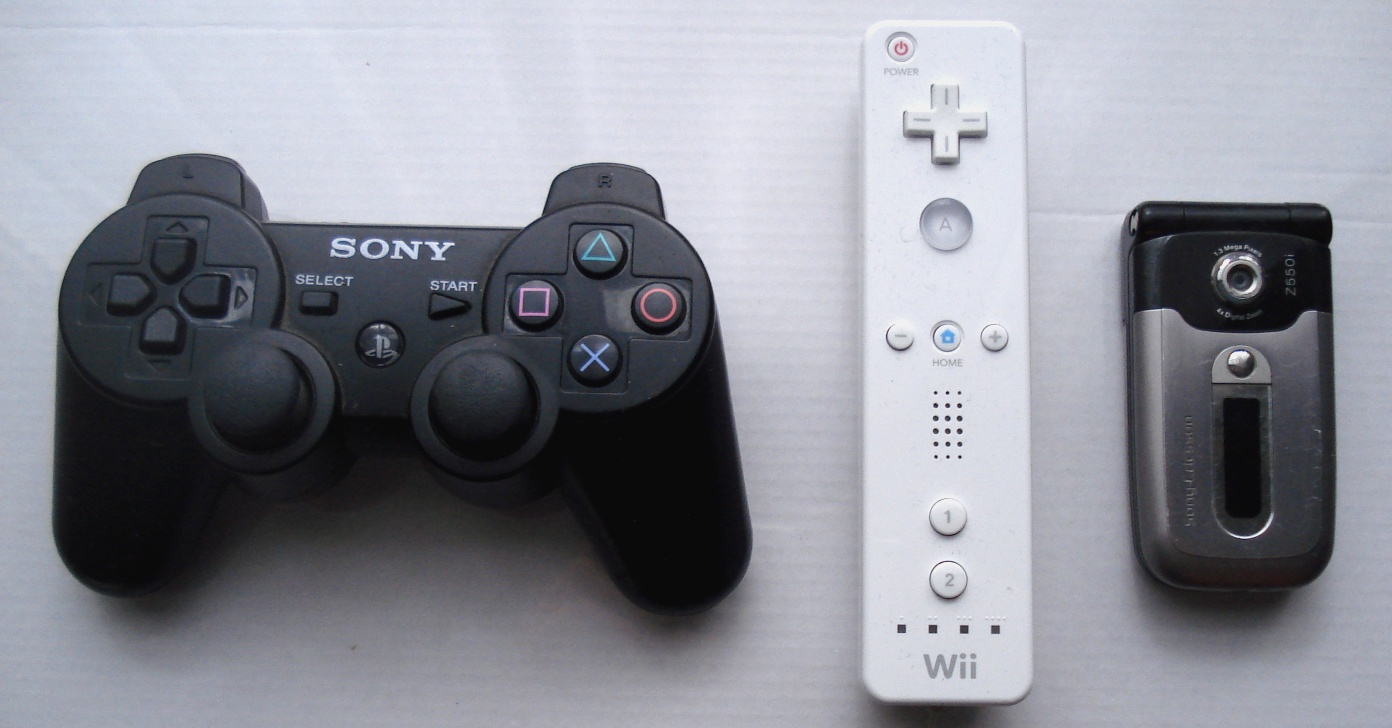
\includegraphics[width=140mm]{BluetoothControllers.jpg}
	\rule{35em}{0.5pt}
	\caption[Tested Working Controllers]{Tested consumer grade Bluetooth enabled devices: \\ Playstation 3 controller \textit{(left)}, Nintendo Wii controller \textit{(middle)}, Sony-Ericsson z550i mobile phone \textit{(right)} }
	\label{fig:workingbtcontrollers}
\end{figure}

All the robot's sensors and other hardware drivers worked correctly, with the user able to control the robot's movement, headlights and horn over both wired USB and wireless Bluetooth HID connections. Sensor data was able to be streamed remotely to a PC or other Bluetooth enabled device supporting the RFCOMM wireless serial port profile. Listing \ref{lst:sensorstream} shows a sample of the streaming sensor data captured from the robot.

\lstinputlisting[float=tbph,caption={Captured RFCOMM streaming sensor data.},label={lst:sensorstream},language={bash}]{./Figures/SensorStream.txt}

A simple C\# application was written to display the streaming sensor data graphically to the user in real time (see Figure \ref{fig:sensorhostapp}). The robot firmware was capable of maintaining both the streaming sensor data connection as well as a secondary connection to a Bluetooth controller simultaneously, allowing for user control of the robot while a PC graphs the retrieved sensor values.

\begin{figure}[tbph]
	\vspace{1em}
	\centering
		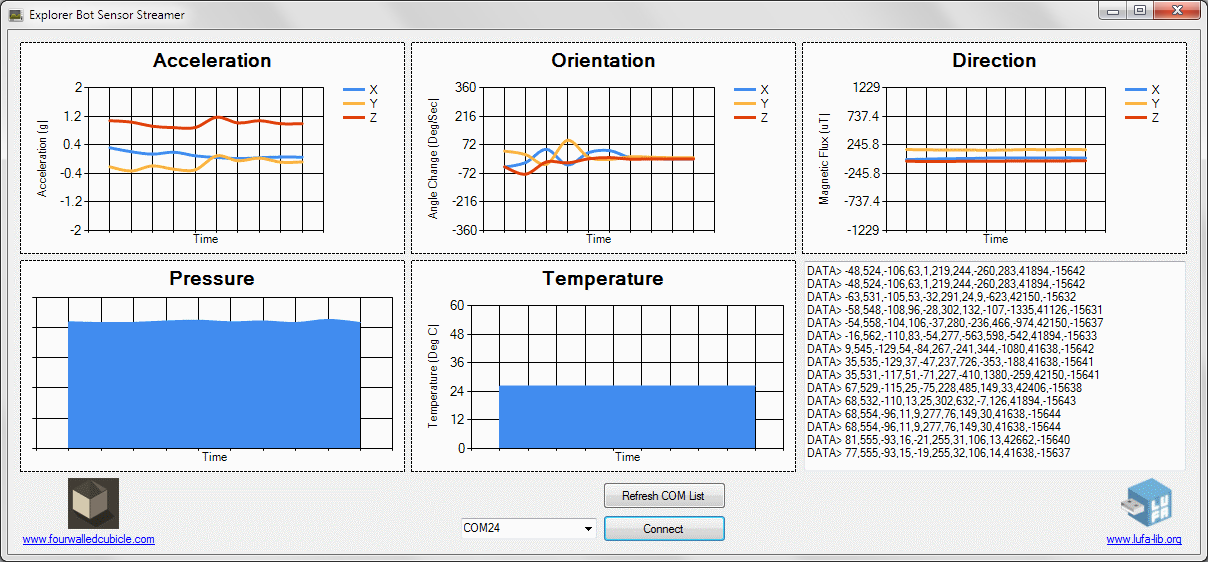
\includegraphics[width=140mm]{SensorDataApp.png}
	\rule{35em}{0.5pt}
	\caption[Sensor Logging Host Application]{Sensor logging application, showing data streaming wirelessly from the connected robot via a Bluetooth virtual serial port. }
	\label{fig:sensorhostapp}
\end{figure}

The completed robot PCB hardware was integrated into a pre-fabricated off-the-shelf robot platform base, and linked to the two wheel mounted DC motors. Additional parts for the PCB retention clip and headlight and horn mounting were designed by the project's Co-Supervisor Robert Ross, and printed out on the University's 3D printer. This resulted in the compact and functional robot prototype shown in Figure \ref{fig:completedrobot}.

\begin{figure}[tbph]
	\vspace{1em}
	\centering
		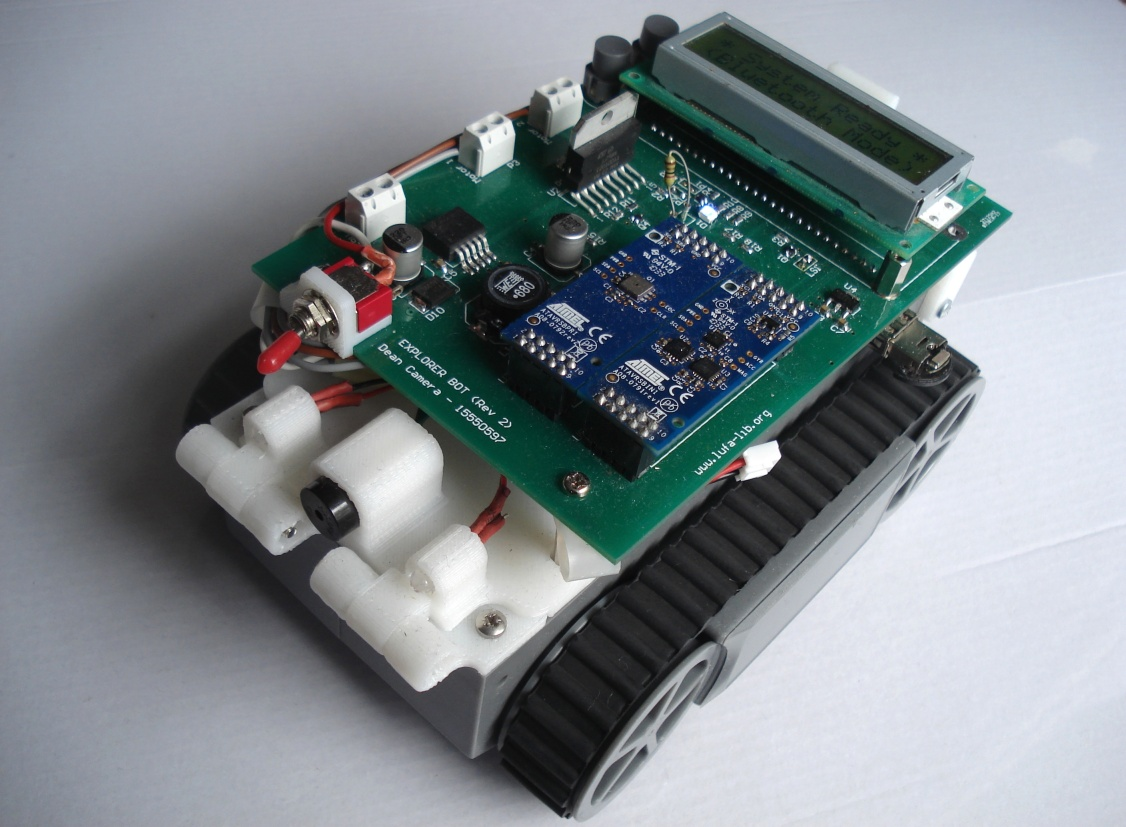
\includegraphics[width=140mm]{CompletedRobot.jpg}
	\rule{35em}{0.5pt}
	\caption[Photo of Completed Robot]{Photo of the completed \textit{ExplorerBot} prototype robot}
	\label{fig:completedrobot}
\end{figure}
	
	\chapter{Project Discussion}
\label{chp:discussion}
\lhead{Chapter \ref{chp:discussion}. \emph{Project Discussion}}

In this chapter, the project's issues (and their solutions) are discussed in detail, as is the implications and impact of the project as a whole. The various phases of the project provided ample opportunities for problem solving, both in hardware and software as the project's development progressed.

\section{Issues Faced}

During the development of the project, as expected a number of issues were faced and overcome. The probability of unexpected issues arising during the development of any non-trivial project rises exponentially with its complexity, and this project was no exception. The main issues are outlined below, along with the solution chosen.

\subsection{Micropendous Pinout PCB Error}

After the manufacture of the first revision PCB was received some weeks after the order was placed, a problem was discovered in the board layout of the main \textit{Micropendous} microcontroller module: the pinouts appeared to have been shifted by one around the entire module perimeter. The root issue cause was traced back to the custom Altium component created for the module; for an explicable reason, Altium begins part component schematic pin numbering from pin 0, instead of the conventional pin 1. This resulted in the pin numbering around the module to be rotated by one place during board layout.

% TODO: Figures showing incorrect and correct pinouts

Coincidentally, as the unroutable pins were marked as \textit{No-Connect} in the robot schematics (due to their unused functions) the Altium DRC module reported no schematic or routing errors. This resulted in the error not being caught until the board manufacturing had been completed, as a cursory visual inspection of the board layout before production did not catch the subtle pin numbering problem.

While it is possible that the board pinouts could be corrected with manual trace cutting and re-wiring, the scale of the error---some forty pins---and the need for other slight board adjustments forced the decision to produce a second, corrected, version of the PCB.

\subsection{Incorrect Transistor Pinout}

During the component ordering phase of the project, an issue was discovered; no NPN transistors could be found in the appropriate SOT-323 footprint that matched the pinouts given by the Altium library component used. To correct this error, it was necessary to mount the transistors flipped upside-down. This inverted orientation corrected the transistor pinouts (see Figure \ref{fig:flippedtransistor}) so that they could be mounted to the board with the application of a small amount of extra solder to bridge the inverted pins to the PCB.

\begin{figure}[H]
	\centering
		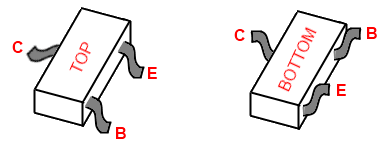
\includegraphics[width=60mm]{FlippedTransistors.png}
	\rule{35em}{0.5pt}
	\caption[Diagram of the normal and flipped SOT-323 Transistor]{Diagram showing the pin-outs of the SOT-323 transistor when mounted normally (\textit{left}) and flipped (\textit{right}).}
	\label{fig:flippedtransistor}
\end{figure}

\subsection{Motor Induced Current Spikes}

During the testing phase of the robot, a failure of the USB AVR microcontroller's USB interface was observed when the motor direction was altered rapidly. Further observation narrowed this down to the switching latency of the chosen inverter transistor (30nS) and H-Bridge (approx. 2$\mu$S). During this time, there exists the possibility of a momentary short in the system battery, if the motor PWM output signal is enabled.

To counteract this, a delay was introduced into the robot's motor driver firmware, to disable the motor output PWM during the switching time. This delay eliminated the high switching current due to the momentary short of the battery, thus preventing the microcontroller USB interface from failing.

Related to the above issue was the motor inrush current, present any time the motor was started from a stationary state. This current, present in all motors under load while the static friction in the motor is overcome, caused large current draw spikes in the main power supply, triggering a destabilization of the main switchmode regulator and thus a brownout of the main microcontroller. This issue was corrected once the main battery was switched from a series of six ``AA'' cell batteries to a much higher rated Lithium-Ion based battery pack.

\subsection{PCA9306 Physical Package}

Despite having some familiarity with hand-soldering somewhat-small multi-pin surface mount IC components, the package used by the PCA9306 I\superscript{2}C level converter presented a serious challenge. This was due to its US-8 package; measuring just 2.7mm x 4.5mm, the component contains eight pins just .3mm wide each.

Rather than risk destroying the component and waiting additional weeks for a replacement, the LaTrobe University Workshop was requested to use a hot-air gun to solder the device to the robot PCB. This ensured that the component would be correctly placed and soldered without a high risk of component damage. In future projects, relatively cheap components such as this should be ordered with one or more extras added to the quantity, so that damaged components (if any) can be replaced immediately without incurring additional delays while new components are ordered. 

\subsection{L298D Unavailability}

In the first PCB revision, the motor controller design centered around the L298D H-Bridge component, which offered logic level inputs, high current/voltage driver outputs, and convenient internal flyback diodes. These flyback diodes---used to dissipate reverse EMF generated by the motor coils' inductance as they are turned on and off---are a critical part of any such circuit involving inductive loads to prevent damage to the driver.

At the time of ordering however, it was discovered that the L298D variant was not readily available from the University's approved component suppliers. As a second revision of the PCB was already required due to the pinout error of the Micropendous module discussed earlier, a set of external flyback diodes were added on the underside of the board, and the L298N H-Bridge IC used as a substitute. Identical in every other way to the L298D, the L298N variant does not contain internal flyback diodes.

\subsection{Unreliable Bluetooth Packet Buffering}

During development, it was found that occasionally packets sent via the Bluetooth interface were (apparently) being ignored by the receiving device --- this was especially apparent during the L2CAP layer channel initialization and configuration phases. In many instances, a channel would fail to configure at all, causing the remote device connection to time out.

After further investigation, it was determined that the problem source was the lack of a reliable packet buffer within the device; if a packet was delayed within the external Bluetooth HCI controller silicon, the controller would reject new packets for transmission. Without a buffer, these rejected packets for transmission would be lost. Ideally, this could be solved by indicating to the controller that only buffer-related event packets should be returned to the host while the controller is busy, to allow for a polled busy-wait scheme to be used to determine the controller's readiness. However, there is no mechanism to delay incoming L2CAP data packets from the controller during this stage in the HCI specifications, which could potentially result in dropped received packets.

To solve this, the stack's L2CAP layer was extended to include its own internal reliable packet transmission scheme, in the form of a small event queue. As channel events were received or generated internally, the pending event would be added to a reliable queue. When a transmission is attempted, these events are only removed from the queue if the transmission was successful (see Chapter \ref{chp:btstackimp}).

This scheme results in a reliable L2CAP layer, without the use of a large internal packet buffer within the device. Additional similar schemes could potentially be added to the higher level service layers, however this was not found to be necessary for the project's firmware.

\subsection{PS3 Controller Compatibility}

Sony's \textit{Playstation 3} controller presented several small difficulties in making it compatible with the rest of the system. While the controller itself implements the standard HID profiles in both wired USB and wireless Bluetooth modes, additional device-specific software tweaks are necessary for compability.

When plugged in as a wired controller via the USB interface, a special HID Feature packet must be sent to the controller over the logical HID interface, via the USB Control endpoint. This packet, directed to the HID report ID \texttt{0xF4} and containing the special ``magic'' bytes \texttt{0x42 0x0C 0x00 0x00}, it is used to enable general controller reports through the regular HID data endpoints. Without this packet, the controller will not send any state change information to the host. In Bluetooth mode, the magic packet required for Bluetooth HID reporting is \texttt{0x42 0x03 0x00 0x00}.

A second packet during initialization is also required, another HID Feature packet directed at the HID Report ID \texttt{0xF5}. Prefixed with the bytes \texttt{0x01 0x00}, this request packet data is followed by the six octets of the host's Bluetooth device address, to pair the controller to the specified address. This is in contrast with the general Bluetooth pairing mechanism, which usually involves a device discovery and authentication phase over the Bluetooth link.

The two initialization packets for USB HID reporting and Bluetooth address pairing are shown in Listing \ref{lst:ps3hidinit}.

\lstinputlisting[float=tbph,caption={Playstation 3 specific initialization code.},label={lst:ps3hidinit}]{./Figures/PS3SpecificInit.c}

\subsection{Misleading Sensor Datasheets}

% TODO

\section{Project Significance}

This project represents a significant impact to the open source and embedded systems communities. It gives a free, open source Bluetooth stack in a new form, paving the way for a new generation of low cost Bluetooth devices. These new devices, using low powered processors previously deemed unsuitable for the task of complex Bluetooth interactions, will give users a new rich landscape of system integration and communication.

While other wireless technologies already in use will remain just as important as they are today, this project gives a new avenue of development for products that can interact directly with off-the-shelf consumer devices. Modern smart-phones, tablet computers and laptops now contain Bluetooth radios as standard features; the stack presented in this project will open up these devices to direct communication with embedded systems without the need for obscure wireless transceiver dongles. In the future, this type of technology will allow for system monitoring and configuration over a wireless link with compatible consumer devices using a rich UI, instead of wired solutions or expensive local displays and buttons.
	\chapter{Conclusion}
\label{chp:conclusion}
\lhead{Chapter \ref{chp:conclusion}. \emph{Conclusion}}

% TODO

\section{Project Success}

% TODO

\section{Future Work}

% TODO

\section{Final Words}

% TODO
%% ----------------------------------------------------------------
\setstretch{1.5}  % Set the line spacing to 1.5, this makes the following tables easier to read
\clearpage  % Start a new page
\lhead{\emph{Abbreviations}}  % Set the left side page header to "Abbreviations"
\listofsymbols{ll}  % Include a list of Abbreviations (a table of two columns)
{
	\textbf{API} & \textbf{A}pplication \textbf{P}rogramming \textbf{I}nterface \\
	\textbf{AVR} & This isn't an acronym. Officially, at least. \\
	\textbf{CPU} & \textbf{C}entral \textbf{P}rocessing \textbf{U}nit \\
	\textbf{DRC} & \textbf{D}esign \textbf{R}ule \textbf{C}heck \\
	\textbf{EEPROM} & \textbf{E}lectrically \textbf{E}rasable \textbf{P}rogrammable \textbf{R}ead \textbf{O}nly \textbf{M}emory \\
	\textbf{FAT} & \textbf{F}ile \textbf{A}llocation \textbf{T}able \\
	\textbf{GPIO} & \textbf{G}eneral \textbf{P}urpose \textbf{I}nput/\textbf{O}utput \\
	\textbf{HCI} & \textbf{H}ost \textbf{C}ontroller \textbf{I}nterface \\
	\textbf{HID} & \textbf{H}uman \textbf{I}nterface \textbf{D}evice \\
	\textbf{IC} & \textbf{I}ntergrated \textbf{C}ircuit \\
	\textbf{I\textsuperscript{2}C} & \textbf{I}nter \textbf{I}ntegrated \textbf{C}ircuit Bus \\
	\textbf{JTAG} & \textbf{J}oint \textbf{T}est \textbf{A}ction \textbf{G}roup \\
	\textbf{L2CAP} & \textbf{L}ogical \textbf{L}ink \textbf{C}ontrol and \textbf{A}daption \textbf{P}rotocol \\
	\textbf{LCD} & \textbf{L}iquid \textbf{C}rystal \textbf{D}isplay \\
	\textbf{LDO} & \textbf{L}ow-\textbf{D}r\textbf{o}pout \\
	\textbf{LED} & \textbf{L}ight \textbf{E}mitting \textbf{D}iode \\
	\textbf{LUFA} & \textbf{L}ightweight \textbf{U}SB \textbf{F}ramework for \textbf{A}VRs \\
	\textbf{PC} & \textbf{P}ersonal \textbf{C}omputer \\
	\textbf{PCB} & \textbf{P}rinted \textbf{C}ircuit \textbf{B}oard \\
	\textbf{PLL} & \textbf{P}hase \textbf{L}ocked \textbf{L}oop \\
	\textbf{PWM} & \textbf{P}ulse \textbf{W}idth \textbf{M}odulation \\
	\textbf{RFCOMM} & \textbf{R}adio \textbf{F}requency \textbf{Comm}unication \\
	\textbf{RTOS} & \textbf{R}eal \textbf{T}ime \textbf{O}perating \textbf{S}ystem \\
	\textbf{SDP} & \textbf{S}ervice \textbf{D}iscovery \textbf{P}rotocol \\
	\textbf{SRAM} & \textbf{S}tatic \textbf{R}andom \textbf{A}ccess \textbf{M}emory \\
	\textbf{TCP/IP} & \textbf{T}ransmission \textbf{C}ontrol \textbf{P}rotocol / \textbf{I}nternet \textbf{P}rotocol \\
	\textbf{UART} & \textbf{U}niversal \textbf{A}synchronous \textbf{R}eceiver \textbf{T}ransmitter \\
	\textbf{UI} & \textbf{U}ser \textbf{I}nterface \\
	\textbf{USB} & \textbf{U}niversal \textbf{S}erial \textbf{B}us \\
}
%% ----------------------------------------------------------------
\addtocontents{toc}{\vspace{1em}} % Add a gap in the Contents, for aesthetics
\appendix % Cue to tell LaTeX that the following 'chapters' are Appendices

	\chapter{Schematics}
\label{Appendix A}
\lhead{Appendix A. \emph{ExplorerBot Robot Schematics}}

\section{Robot Schematics}

The following pages illustrate the complete schematics of the \emph{ExplorerBot} robot hardware created to demonstrate a practical application of the Bluetooth stack.

\includepdf[pages=4, landscape, offset=80 -70]{./Appendices/Schematics.pdf}
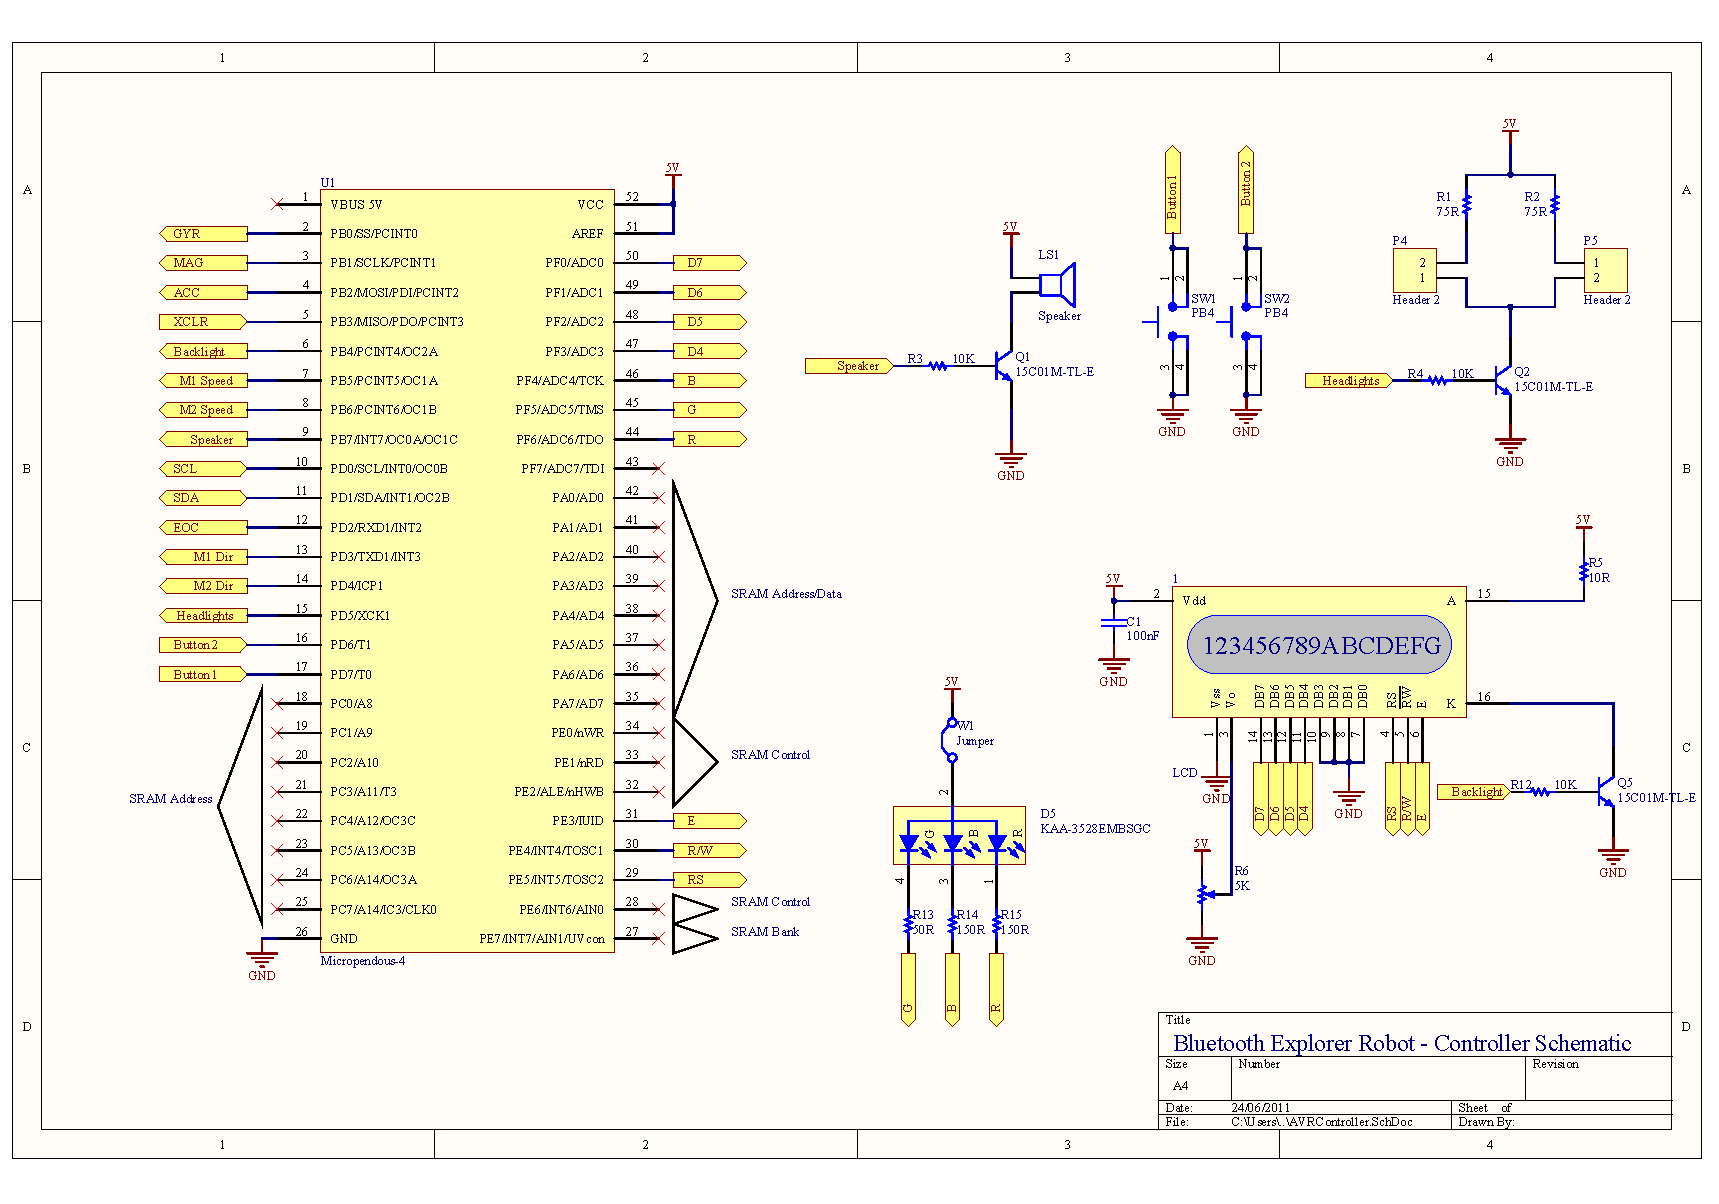
\includepdf[pages={1-3}, landscape, offset=80 -70]{./Appendices/Schematics.pdf}
\includepdf[pages=5, landscape, offset=80 -70]{./Appendices/Schematics.pdf}
	\chapter{Source Code}
\label{app:sourcecode}
\lhead{Appendix \ref{app:sourcecode}. \emph{Source Code}}

The complete project source code is available for download online, due to its significant size. Both the robot firmware and the embedded Bluetooth stack may be viewed and modified according to the licence agreements included at the top of each source file in the download package.

\section{Obtaining the Source Code}

All relevant material relating to this project (including source code, schematics, and this document) may be obtained from the official project page, located at \\ \href{http://www.fourwalledcubicle.com/ExplorerBot.php}{\textit{http://www.fourwalledcubicle.com/ExplorerBot.php}}.

\section{Build Dependencies}

The Bluetooth stack and robot firmware was written in the C language, and targeted at the free open source AVR-GCC compiler and avr-libc library. A standard \texttt{makefile} included with the firmware allows for command line control over the building of the project files into a set of binaries which can then be programmed into the target microcontroller for use via the command \texttt{make all}. The following tools are required to build the firmware under Windows:

\begin{itemize}
	\item The \textbf{WinAVR 20100101} release download, or Windows binaries of the \textbf{GNU Shell Utilities}
	\item The latest \textbf{AVR Toolchain} release download from Atmel (included with Atmel's free \textit{AVRStudio 5} software)
\end{itemize}

Under Debian Linux environments, the following packages are required:

\begin{itemize}
	\item \textbf{gcc-avr} 
	\item \textbf{binutils-avr}
	\item \textbf{avr-libc}
	\item \textbf{avrdude}
\end{itemize}

Which can be installed via the command prompt using the command \texttt{sudo apt-get install gcc-avr binutils-avr avr-libc avrdude}.
	\chapter{Robot User Guide}
\label{app:robotuserguide}
\lhead{Appendix \ref{app:robotuserguide}. \emph{Robot User Guide}}

% TODO

\section{Power Requirements}

% TODO

\section{Supported USB Devices}

% TODO

\subsection{HID Class Devices}

% TODO

\subsection{Mass Storage Class Devices}

% TODO

\subsection{Bluetooth Adapter Devices}

% TODO

\section{Supported Bluetooth Services}

% TODO

\subsection{HID Service}

% TODO

\subsection{RFCOMM Service}

% TODO
	
\addtocontents{toc}{\vspace{2em}}  % Add a gap in the Contents, for aesthetics
\backmatter
%% ----------------------------------------------------------------
\label{Bibliography}
\lhead{\emph{Bibliography}}  % Change the left side page header to "Bibliography"
\bibliographystyle{unsrtnat}  % Use the "unsrtnat" BibTeX style for formatting the Bibliography
\bibliography{Thesis}  % The references (bibliography) information are stored in the file named "Bibliography.bib"
%% ----------------------------------------------------------------
\end{document}  % The End
